% Vietnamese pdfLaTeX build
\documentclass[11pt,a4paper]{article}

\usepackage[utf8]{vntex,inputenc}
\usepackage[T5]{fontenc}
\usepackage{amsmath,amssymb,mathtools}
\usepackage{geometry}
\usepackage{setspace}
\usepackage{enumitem}
\usepackage{needspace}
\usepackage{titlesec}
\usepackage{fancyhdr}
\usepackage{microtype}
\usepackage{circuitikz}
\usepackage{pgfplots}
\pgfplotsset{compat=1.18}
\usetikzlibrary{arrows.meta,calc,positioning,decorations.pathmorphing}
\usepackage[hidelinks]{hyperref}

\geometry{left=1.85cm,right=1.85cm,top=1.65cm,bottom=1.55cm,headheight=16pt,headsep=0.35cm,footskip=0.75cm}
\setstretch{1.06}
\setlength{\parindent}{0pt}
\setlength{\parskip}{0.22em}
\setlength{\abovedisplayskip}{5pt plus 1pt minus 2pt}
\setlength{\belowdisplayskip}{5pt plus 1pt minus 2pt}
\setlength{\abovedisplayshortskip}{3pt plus 1pt}
\setlength{\belowdisplayshortskip}{3pt plus 1pt minus 1pt}
\setlength{\jot}{2pt}
\raggedbottom
\setlist[itemize]{leftmargin=1.6em,itemsep=0.2em,topsep=0.2em}
\allowdisplaybreaks

\pagestyle{fancy}
\fancyhf{}
\fancyhead[L]{\small\sffamily LÝ THUYẾT ĐIỀU KHIỂN TỰ ĐỘNG}
\fancyhead[R]{\small\sffamily Bài tập và lời giải}
\fancyfoot[C]{\thepage}
\renewcommand{\headrulewidth}{0.3pt}

\titleformat{\section}{\large\bfseries}{}{0pt}{}
\titlespacing*{\section}{0pt}{0.75em}{0.2em}

\newcommand{\baitap}[1]{%
  \Needspace{4\baselineskip}%
  \section*{Bài #1}%
}
\newcommand{\debai}{\par\noindent\textbf{Đề bài.}\enspace}
\newcommand{\loigiai}{\par\smallskip\noindent\textbf{Lời giải.}\enspace}
\newcommand{\Lap}{\mathcal{L}}
\newcommand{\chuong}[2]{%
  \par\medskip
  \noindent{\Large\bfseries CHƯƠNG #1 -- #2}\par
  \smallskip\hrule\medskip
}
\tikzset{
  block/.style={draw,rectangle,minimum width=1.7cm,minimum height=0.75cm,align=center},
  sum/.style={draw,circle,minimum size=6.5mm,inner sep=0pt},
  pickoff/.style={circle,fill,inner sep=1.3pt}
}

\begin{document}

\noindent{\bfseries\large BÀI TẬP VÀ LỜI GIẢI -- LÝ THUYẾT ĐIỀU KHIỂN TỰ ĐỘNG}
\vspace{0.25em}
\hrule
\vspace{0.45em}

\chuong{2}{MÔ HÌNH TOÁN HỌC CỦA HỆ THỐNG}

\baitap{2.1}
\debai
Tìm biến đổi Laplace ngược của
\[
F(s)=\frac{1}{s^2-8s+7}.
\]

\loigiai
Phân tích mẫu số:
\[
s^2-8s+7=(s-1)(s-7).
\]
Do đó
\[
F(s)=\frac{1}{(s-1)(s-7)}
=\frac{C_1}{s-1}+\frac{C_2}{s-7}.
\]
Với các cực đơn, dùng
\[
C_i=\left[(s-p_i)F(s)\right]_{s=p_i}.
\]
Suy ra
\[
C_1=\left[\frac{1}{s-7}\right]_{s=1}=-\frac16,
\qquad
C_2=\left[\frac{1}{s-1}\right]_{s=7}=\frac16.
\]
Vậy
\[
F(s)=-\frac{1}{6}\frac{1}{s-1}+\frac{1}{6}\frac{1}{s-7}.
\]
Dùng
\[
\Lap^{-1}\left\{\frac{1}{s-a}\right\}=e^{at}1(t),
\]
ta được
\[
\boxed{f(t)=\frac{e^{7t}-e^t}{6}\,1(t)}.
\]

\baitap{2.2}
\debai
Giải phương trình vi phân
\[
\frac{d^2y}{dt^2}-8\frac{dy}{dt}+7y=4,
\qquad y(0)=0,\quad y'(0)=0.
\]

\loigiai
Lấy biến đổi Laplace hai vế. Với bài toán một phía ($t\ge 0$), hằng số $4$ được hiểu là $4\,1(t)$ nên
\[
\Lap\{4\}=4\Lap\{1(t)\}=\frac{4}{s}.
\]
Công thức tổng quát cho đạo hàm là
\[
\Lap\{y'\}=sY(s)-y(0),\qquad
\Lap\{y''\}=s^2Y(s)-sy(0)-y'(0).
\]
Do $y(0)=0$ và $y'(0)=0$,
\[
\Lap\{y'\}=sY(s),\qquad \Lap\{y''\}=s^2Y(s).
\]
Suy ra
\[
s^2Y(s)-8sY(s)+7Y(s)=\frac4s,
\]
hay
\[
Y(s)=\frac{4}{s(s^2-8s+7)}
=\frac{4}{s(s-1)(s-7)}.
\]
Tách phân thức:
\[
Y(s)=\frac{C_1}{s}+\frac{C_2}{s-1}+\frac{C_3}{s-7}.
\]
Các hệ số là
\[
C_1=\left[sY(s)\right]_{s=0}=\frac47,
\]
\[
C_2=\left[(s-1)Y(s)\right]_{s=1}=-\frac23,
\]
\[
C_3=\left[(s-7)Y(s)\right]_{s=7}=\frac{2}{21}.
\]
Do đó
\[
Y(s)=\frac47\frac1s-\frac23\frac1{s-1}+\frac{2}{21}\frac1{s-7}.
\]
Lấy Laplace ngược:
\[
\boxed{y(t)=\left(\frac47-\frac23e^t+\frac{2}{21}e^{7t}\right)1(t)}.
\]

\baitap{2.3}
\debai
Giả sử $F(s)$ có một cực bội bậc $3$ tại $s=p$ và phần phân thức tương ứng có dạng
\[
F(s)=\frac{C_1}{(s-p)^3}+\frac{C_2}{(s-p)^2}+\frac{C_3}{s-p}+\cdots.
\]
Suy ra công thức xác định $C_1,C_2,C_3$.

\loigiai
Nhân hai vế với $(s-p)^3$:
\[
(s-p)^3F(s)=C_1+C_2(s-p)+C_3(s-p)^2+\cdots.
\]
Cho $s=p$:
\[
\boxed{C_1=\left[(s-p)^3F(s)\right]_{s=p}}.
\]
Lấy đạo hàm theo $s$:
\[
\frac{d}{ds}\big[(s-p)^3F(s)\big]
=C_2+2C_3(s-p)+\cdots.
\]
Cho $s=p$:
\[
\boxed{C_2=\left[\frac{d}{ds}\big((s-p)^3F(s)\big)\right]_{s=p}}.
\]
Lấy đạo hàm lần hai:
\[
\frac{d^2}{ds^2}\big[(s-p)^3F(s)\big]=2C_3+\cdots.
\]
Vì vậy
\[
\boxed{C_3=\frac{1}{2!}\left[\frac{d^2}{ds^2}\big((s-p)^3F(s)\big)\right]_{s=p}}.
\]

\baitap{2.4}
\debai
Giải phương trình
\[
\frac{dy(t)}{dt}+4y(t)=5u_{in}(t),
\]
trong đó $u_{in}(t)=1(t)$ và $y(0)=0$.

\loigiai
Vì
\[
\Lap\{1(t)\}=\frac1s,
\]
nên
\[
sY(s)-y(0)+4Y(s)=\frac5s.
\]
Thay $y(0)=0$:
\[
(s+4)Y(s)=\frac5s
\quad\Rightarrow\quad
Y(s)=\frac{5}{s(s+4)}.
\]
Tách phân thức:
\[
\frac{5}{s(s+4)}=\frac{A}{s}+\frac{B}{s+4}.
\]
Nhân với $s(s+4)$:
\[
5=A(s+4)+Bs.
\]
Cho $s=0$ và $s=-4$:
\[
A=\frac54,\qquad B=-\frac54.
\]
Vậy
\[
Y(s)=\frac54\frac1s-\frac54\frac1{s+4},
\]
và
\[
\boxed{y(t)=\frac54\left(1-e^{-4t}\right)1(t)}.
\]

\baitap{2.5}
\debai
Cho
\[
F(s)=\frac{s+5}{s+1},\qquad s=-1+j3.
\]
Tính giá trị phức, biên độ và pha của $F(s)$.

\loigiai
Thay $s=-1+j3$:
\[
F(-1+j3)=\frac{4+j3}{j3}=1-\frac43j.
\]
Biên độ:
\[
|F|=\sqrt{1^2+\left(-\frac43\right)^2}=\frac53.
\]
Pha:
\[
\varphi=\tan^{-1}\left(-\frac43\right)\approx -53.13^\circ.
\]
Do đó
\[
\boxed{F(-1+j3)=1-\frac43j=\frac53\angle(-53.13^\circ)}.
\]

\baitap{2.6}
\debai
Tìm biến đổi Laplace của
\[
f(t)=t^2+e^{-2t}\sin 3t.
\]

\loigiai
Theo tính tuyến tính,
\[
F(s)=\Lap\{t^2\}+\Lap\{e^{-2t}\sin3t\}.
\]
Với
\[
\Lap\{t^n\}=\frac{n!}{s^{n+1}},
\]
ta có
\[
\Lap\{t^2\}=\frac{2}{s^3}.
\]
Mặt khác,
\[
\Lap\{\sin3t\}=\frac{3}{s^2+9}.
\]
Dùng tính chất dịch
\[
e^{-at}f(t)\ \longleftrightarrow\ F(s+a),
\]
suy ra
\[
\Lap\{e^{-2t}\sin3t\}=\frac{3}{(s+2)^2+9}.
\]
Vậy
\[
\boxed{F(s)=\frac{2}{s^3}+\frac{3}{(s+2)^2+9}}.
\]

\baitap{2.7}
\debai
Tìm biến đổi Laplace của
\[
f(t)=t\sin t.
\]

\loigiai
Dùng tính chất
\[
\Lap\{tf(t)\}=-\frac{d}{ds}F(s),
\qquad F(s)=\Lap\{f(t)\}.
\]
Vì
\[
\Lap\{\sin t\}=\frac{1}{s^2+1},
\]
nên
\[
\Lap\{t\sin t\}
=-\frac{d}{ds}\left(\frac{1}{s^2+1}\right)
=\frac{2s}{(s^2+1)^2}.
\]
Do đó
\[
\boxed{\Lap\{t\sin t\}=\frac{2s}{(s^2+1)^2}}.
\]

\baitap{2.8}
\debai
Tìm biến đổi Laplace ngược của
\[
F(s)=\frac{2(s^2+s+1)}{s(s+1)^2}.
\]

\loigiai
Do $s=-1$ là cực bội bậc $2$, đặt
\[
F(s)=\frac{C_1}{s}+\frac{C_2}{s+1}+\frac{C_3}{(s+1)^2}.
\]
Với cực đơn $s=0$:
\[
C_1=\left[sF(s)\right]_{s=0}=2.
\]
Với cực bội $s=-1$:
\[
C_3=\left[(s+1)^2F(s)\right]_{s=-1}
=\left[\frac{2(s^2+s+1)}{s}\right]_{s=-1}=-2.
\]
Đặt
\[
H(s)=(s+1)^2F(s)=2\left(s+1+\frac1s\right).
\]
Khi đó
\[
C_2=H'(-1)
=\left[2\left(1-\frac1{s^2}\right)\right]_{s=-1}=0.
\]
Vậy
\[
F(s)=\frac2s-\frac{2}{(s+1)^2}.
\]
Dùng
\[
\Lap^{-1}\left\{\frac{1}{(s+a)^2}\right\}=te^{-at}1(t),
\]
ta được
\[
\boxed{f(t)=\left(2-2te^{-t}\right)1(t)}.
\]

\baitap{2.9}
\debai
Một xe được mô hình hóa bởi khối lượng $m$ và hệ số ma sát nhớt $b$. Lực kéo là $u(t)$, độ dịch chuyển là $d(t)$. Cho
\[
m=b=1,\qquad u(t)=1(t),\qquad d(0)=0,\quad \dot d(0)=0.
\]
Hãy tìm hàm truyền $G(s)=D(s)/U(s)$ và đáp ứng $d(t)$.

\loigiai
Theo định luật II Newton,
\[
\sum F=ma.
\]
Lực ma sát nhớt là $b\dot d(t)$, ngược chiều chuyển động, nên
\[
u(t)-b\dot d(t)=m\ddot d(t).
\]
Hay
\[
m\ddot d(t)+b\dot d(t)=u(t).
\]
Lấy Laplace với điều kiện đầu bằng không:
\[
(ms^2+bs)D(s)=U(s).
\]
Do đó
\[
\boxed{G(s)=\frac{D(s)}{U(s)}=\frac{1}{ms^2+bs}}.
\]
Với $m=b=1$:
\[
G(s)=\frac{1}{s(s+1)}.
\]
Vì $u(t)=1(t)$ nên $U(s)=1/s$, do đó
\[
D(s)=G(s)U(s)=\frac{1}{s^2(s+1)}.
\]
Tách phân thức:
\[
D(s)=-\frac1s+\frac1{s^2}+\frac1{s+1}.
\]
Lấy Laplace ngược:
\[
\boxed{d(t)=\left(-1+t+e^{-t}\right)1(t)}.
\]

\baitap{2.10}
\debai
Xét con lắc đơn có khối lượng $m$, chiều dài $l$, góc lệch $\theta$ so với phương thẳng đứng và mômen điều khiển $T_c$. Hãy lập mô hình phi tuyến và tuyến tính hóa quanh điểm làm việc $\theta=0$.

\begin{center}
\begin{tikzpicture}[scale=1.05,>=Stealth]
  \coordinate (O) at (0,2.75);
  \coordinate (P) at ({2.45*sin(28)},{2.75-2.45*cos(28)});
  \coordinate (V) at (0,0.05);
  \draw[thick] (-1.2,3.15)--(1.2,3.15);
  \draw[fill=black] (O) circle (1.5pt);
  \draw[dashed] (O)--(V);
  \draw[very thick] (O)--(P) node[midway,right]{$l$};
  \draw[fill=black] (P) circle (2.7pt);
  \node[above left] at (O) {O};

  % Quy ước: theta dương theo chiều kim đồng hồ từ phương thẳng đứng xuống.
  \draw[->,thick,blue] ($(O)+(0,-0.85)$) arc[start angle=-90,end angle=-62,radius=0.85];
  \node[blue] at ($(O)+(0.38,-0.92)$) {$\theta$};

  % Mômen điều khiển T_c cùng chiều dương của theta.
  \draw[->,thick] ($(O)+(0.72,0.05)$) arc[start angle=8,end angle=-62,radius=0.72];
  \node[right] at ($(O)+(0.78,0.32)$) {$T_c$};

  % Trọng lực và thành phần tiếp tuyến gây mômen hồi phục.
  \draw[->,thick,red] (P)--++(0,-1.35) node[right]{$mg$};
  \draw[->,thick,red!70!black] (P)--++({-0.95*cos(28)},{-0.95*sin(28)})
    node[below left]{$mg\sin\theta$};
  \node[align=left] at (3.45,1.85) {chiều dương $\theta$\\và $T_c$};
\end{tikzpicture}
\end{center}

\loigiai
Mômen quán tính của vật đối với điểm treo là
\[
I=ml^2.
\]
Chọn chiều dương của $\theta$ theo chiều kim đồng hồ từ phương thẳng đứng xuống và chọn $T_c$ dương cùng chiều đó. Tổng mômen quanh điểm treo bằng mômen quán tính nhân gia tốc góc:
\[
\sum M_O = I\ddot\theta.
\]
Thành phần tiếp tuyến $mg\sin\theta$ tạo mômen hồi phục ngược chiều dương nên mômen trọng lực là $-mgl\sin\theta$. Mômen điều khiển là $+T_c$. Do đó
\[
T_c-mgl\sin\theta=ml^2\ddot\theta.
\]
Chia cả hai vế cho $ml^2$ thu được mô hình phi tuyến:
\[
\boxed{\ddot\theta+\frac{g}{l}\sin\theta=\frac{T_c}{ml^2}}.
\]
Để tuyến tính hóa quanh $\theta=0$, dùng khai triển Taylor của $\sin\theta$ tại $0$:
\[
\sin\theta\approx \sin0+\cos0\,\theta=\theta.
\]
Suy ra mô hình tuyến tính hóa:
\[
\boxed{\ddot\theta+\frac{g}{l}\theta=\frac{T_c}{ml^2}}.
\]

\baitap{2.11}
\debai
Xét mạch dẫn trước (lead network) như hình dưới. Giữa nút vào và nút $A$ có hai nhánh song song: nhánh trên là tụ $C$, nhánh dưới là điện trở $R_1$. Từ nút $A$ xuống mass là điện trở $R_2$. Tìm hàm truyền
\[
G(s)=\frac{V_{out}(s)}{V_{in}(s)},
\]
biết $v_C(0)=0$.

\begin{center}
\begin{circuitikz}[european resistors, scale=1.0, transform shape]
  \coordinate (IN) at (0,3.2);
  \coordinate (GND) at (0,0);
  \coordinate (A) at (5.4,3.2);
  \coordinate (B) at (5.4,0);

  % Hai nhánh song song từ nút vào đến A: C và R1.
  \draw (IN) node[circ]{} to[R=$R_1$] (A) node[circ,label=above:$A$]{};
  \draw (IN) -- (0,4.45) to[C=$C$] (5.4,4.45) -- (A);

  % Nhánh ra R2 và dây hồi về nút âm của Vin.
  \draw (A) to[R,l_=$R_2$] (B) node[circ]{} -- (GND) node[circ]{};
  \draw (B) node[ground]{};

  % Cực tính điện áp đúng theo ghi chép gốc:
  % Vin: + ở nút trên, - ở nút dưới.
  \node[left] at ($(IN)+(-0.15,0.18)$) {$+$};
  \node[left] at ($(GND)+(-0.15,-0.18)$) {$-$};
  \node[left] at (-0.55,1.6) {$V_{in}$};

  % vC: + bên trái tụ, - bên phải tụ.
  \node[above] at ($(IN)+(1.55,1.25)$) {$+$};
  \node[above] at ($(A)+(-1.55,1.25)$) {$-$};

  % Vout: + tại A, - tại nút dưới.
  \node[right] at ($(A)+(0.18,0.18)$) {$+$};
  \node[right] at ($(B)+(0.18,-0.18)$) {$-$};
  \node[right] at (6.35,1.6) {$V_{out}$};

  % Chiều dòng điện: iC, iR1 sang phải; iR2 đi xuống.
  \draw[->,thick] (1.05,4.70)--(2.05,4.70) node[midway,above]{$i_C$};
  \draw[->,thick] (1.25,3.52)--(2.25,3.52) node[midway,above]{$i_{R_1}$};
  \draw[->,thick] (5.90,2.85)--(5.90,1.95) node[midway,right]{$i_{R_2}$};

  % Vòng KVL I theo chiều kim đồng hồ.
  \draw[->,thick] (2.10,1.20) arc[start angle=205,end angle=-120,radius=0.72];
  \node at (2.10,1.20) {$I$};
\end{circuitikz}
\end{center}

\loigiai
Tại nút $A$, áp dụng định luật Kirchhoff dòng điện (KCL):
\[
i_C+i_{R_1}=i_{R_2}.
\]
Với quy ước cực tính trên hình, dòng $i_C$ và $i_{R_1}$ đi từ cực dương sang cực âm của $v_C$, còn $i_{R_2}$ đi từ cực dương sang cực âm của $v_{out}$. Do đó
\[
i_C=C\frac{dv_C}{dt},\qquad
i_{R_1}=\frac{v_C}{R_1},\qquad
i_{R_2}=\frac{v_{out}}{R_2}.
\]
Suy ra
\[
C\frac{dv_C}{dt}+\frac{v_C}{R_1}=\frac{v_{out}}{R_2}. \tag{1}
\]
Theo KVL trên vòng $I$:
\[
v_C+v_{out}-v_{in}=0,
\]
hay
\[
v_C=v_{in}-v_{out}. \tag{2}
\]
Lấy biến đổi Laplace của (1), với $v_C(0)=0$:
\[
\left(sC+\frac1{R_1}\right)V_C(s)=\frac{V_{out}(s)}{R_2}. \tag{3}
\]
Từ (2):
\[
V_C(s)=V_{in}(s)-V_{out}(s). \tag{4}
\]
Thay (4) vào (3):
\[
\left(sC+\frac1{R_1}\right)\big(V_{in}-V_{out}\big)=\frac{V_{out}}{R_2}.
\]
Sắp xếp lại:
\[
\left(sC+\frac1{R_1}\right)V_{in}
=
\left(sC+\frac1{R_1}+\frac1{R_2}\right)V_{out}.
\]
Vì vậy
\[
\boxed{
G(s)=\frac{V_{out}(s)}{V_{in}(s)}
=
\frac{sC+\dfrac1{R_1}}
{sC+\dfrac1{R_1}+\dfrac1{R_2}}
}.
\]
Chia cả tử và mẫu cho $C$:
\[
\boxed{
G(s)=
\frac{s+\dfrac1{R_1C}}
{s+\dfrac1{R_1C}+\dfrac1{R_2C}}
}.
\]
Nếu đặt
\[
b=\frac1{R_1C},\qquad
a=\frac1{R_1C}+\frac1{R_2C},
\]
thì
\[
\boxed{G(s)=\frac{s+b}{s+a}},\qquad b<a.
\]

\baitap{2.12}
\debai
(Buổi 4 -- câu a) Giải phương trình vi phân
\[
\boxed{y''-7y'-8y=10e^t},
\]
với
\[
y(0)=1,\qquad y'(0)=3.
\]
Tìm $y(t)$.

\loigiai
Lấy Laplace hai vế:
\[
\Lap\{y''\}=s^2Y(s)-sy(0)-y'(0)=s^2Y(s)-s-3,
\]
\[
\Lap\{-7y'\}=-7[sY(s)-y(0)]=-7sY(s)+7,
\]
\[
\Lap\{-8y\}=-8Y(s),
\]
và
\[
\Lap\{10e^t\}=\frac{10}{s-1}.
\]
Do đó
\[
s^2Y-s-3-7sY+7-8Y=\frac{10}{s-1}.
\]
Nhóm các số hạng chứa $Y(s)$:
\[
(s^2-7s-8)Y(s)-s+4=\frac{10}{s-1}.
\]
Suy ra
\[
(s^2-7s-8)Y(s)=\frac{10}{s-1}+s-4,
\]
\[
Y(s)=\frac{\dfrac{10}{s-1}+s-4}{s^2-7s-8}.
\]
Phân tích mẫu:
\[
s^2-7s-8=(s-8)(s+1).
\]
Quy đồng tử:
\[
\frac{10}{s-1}+s-4
=\frac{10+(s-4)(s-1)}{s-1}
=\frac{s^2-5s+14}{s-1}.
\]
Vì vậy
\[
\boxed{
Y(s)=\frac{s^2-5s+14}{(s-1)(s-8)(s+1)}
}.
\]
Tách phân thức:
\[
Y(s)=\frac{A}{s-1}+\frac{B}{s-8}+\frac{C}{s+1}.
\]
Với $A$:
\[
A=\left[(s-1)Y(s)\right]_{s=1}
=\frac{1^2-5(1)+14}{(1-8)(1+1)}
=-\frac57.
\]
Với $B$:
\[
B=\left[(s-8)Y(s)\right]_{s=8}
=\frac{8^2-5(8)+14}{(8-1)(8+1)}
=\frac{38}{63}.
\]
Với $C$:
\[
C=\left[(s+1)Y(s)\right]_{s=-1}
=\frac{(-1)^2-5(-1)+14}{(-1-1)(-1-8)}
=\frac{10}{9}.
\]
Do đó
\[
Y(s)=-\frac57\frac1{s-1}
+\frac{38}{63}\frac1{s-8}
+\frac{10}{9}\frac1{s+1}.
\]
Lấy Laplace ngược:
\[
\boxed{
y(t)=-\frac57e^t+\frac{38}{63}e^{8t}+\frac{10}{9}e^{-t}
}.
\]
Kiểm tra điều kiện đầu:
\[
y(0)=-\frac57+\frac{38}{63}+\frac{10}{9}=1,
\]
\[
y'(0)=-\frac57+8\cdot\frac{38}{63}-\frac{10}{9}=3.
\]


\baitap{2.13}
\debai
(Buổi 4 -- ví dụ mạch điện) Xét mạch gồm nguồn điện áp $v(t)$, điện trở $R_1$, cuộn cảm $L$, điện trở $R_2$ và tụ điện $C$ như hình. Hai dòng vòng được chọn là $i_1(t)$ và $i_2(t)$, cùng chiều kim đồng hồ. Hãy tìm hàm truyền
\[
\boxed{G(s)=\frac{I_2(s)}{V(s)}}
\]
với giả thiết
\[
v_C(0)=0,\qquad i_L(0)=0.
\]

\begin{center}
\begin{circuitikz}[european resistors, scale=1.0, transform shape, >=Stealth]
  \coordinate (BL) at (0,0);
  \coordinate (TL) at (0,3.1);
  \coordinate (A)  at (4.0,3.1);
  \coordinate (B)  at (4.0,0);
  \coordinate (TR) at (8.0,3.1);
  \coordinate (BR) at (8.0,0);

  \draw (BL) to[sV,l_=$v(t)$] (TL)
        to[R=$R_1$] (A) node[circ,label=above:$A$]{}
        to[R=$R_2$] (TR)
        to[C=$C$] (BR)
        -- (B) node[circ,label=below:$B$]{}
        -- (BL);

  \draw (A) to[L=$L$] (B);

  % Dòng vòng: cùng chiều kim đồng hồ.
  \draw[->,thick] (1.15,1.50) arc[start angle=160,end angle=-155,radius=0.62];
  \node at (1.15,1.50) {$i_1(t)$};

  \draw[->,thick] (6.15,1.50) arc[start angle=160,end angle=-155,radius=0.62];
  \node at (6.15,1.50) {$i_2(t)$};

  % Điện áp tụ theo quy ước thụ động.
  \node[right] at ($(TR)+(0.20,-0.25)$) {$+$};
  \node[right] at ($(BR)+(0.20,0.25)$) {$-$};
  \node[right] at (8.55,1.55) {$v_C(t)$};
\end{circuitikz}
\end{center}

\loigiai
Ta giải đúng theo hai dòng vòng trong hình ghi chép. Vì $i_1$ và $i_2$ cùng chiều kim đồng hồ nên trên nhánh chung chứa cuộn cảm, dòng thực theo chiều từ $A$ xuống $B$ là
\[
i_L=i_1-i_2.
\]

\textbf{Cách 1: lập phương trình KVL trong miền thời gian rồi biến đổi Laplace.}

Vòng I:
\[
u_{R_1}+u_L-v=0.
\]
Với
\[
u_{R_1}=R_1i_1,\qquad
u_L=L\frac{d}{dt}(i_1-i_2),
\]
ta được
\[
R_1i_1+L\left(\frac{di_1}{dt}-\frac{di_2}{dt}\right)=v(t). \tag{1}
\]

Vòng II:
\[
u_{R_2}+u_C-u_L=0.
\]
Do
\[
u_{R_2}=R_2i_2,\qquad
u_C=\frac1C\int_0^t i_2(\tau)\,d\tau,
\]
nên
\[
R_2i_2+\frac1C\int_0^t i_2(\tau)\,d\tau
+L\left(\frac{di_2}{dt}-\frac{di_1}{dt}\right)=0. \tag{2}
\]

Vì $v_C(0)=0$ và $i_L(0)=0$, biến đổi Laplace của (1), (2) cho:
\[
R_1I_1(s)+Ls\big[I_1(s)-I_2(s)\big]=V(s), \tag{3}
\]
\[
R_2I_2(s)+\frac{1}{Cs}I_2(s)
+Ls\big[I_2(s)-I_1(s)\big]=0. \tag{4}
\]

Từ (4):
\[
Ls\,I_1(s)
=
\left(R_2+\frac1{Cs}+Ls\right)I_2(s),
\]
do đó
\[
I_1(s)
=
\left(
1+\frac{R_2}{Ls}+\frac{1}{LCs^2}
\right)I_2(s). \tag{5}
\]

Thay (5) vào (3):
\[
(R_1+Ls)I_1-LsI_2=V.
\]
Suy ra
\[
\left[
R_1+R_2+\frac{R_1R_2}{Ls}
+\frac{R_1}{LCs^2}
+\frac1{Cs}
\right]I_2(s)=V(s).
\]
Nhân cả tử và mẫu với $LCs^2$:
\[
\boxed{
G(s)=\frac{I_2(s)}{V(s)}
=
\frac{LCs^2}
{(R_1+R_2)LCs^2+(R_1R_2C+L)s+R_1}
}.
\]

\textbf{Cách 2: thay trực tiếp các phần tử bởi trở kháng trong miền $s$.}

Với điều kiện đầu bằng không:
\[
Z_{R_1}=R_1,\qquad
Z_{R_2}=R_2,\qquad
Z_L=Ls,\qquad
Z_C=\frac1{Cs}.
\]
Hai phương trình dòng vòng trong miền $s$ là
\[
(R_1+Ls)I_1-LsI_2=V, \tag{6}
\]
\[
-LsI_1+\left(R_2+\frac1{Cs}+Ls\right)I_2=0. \tag{7}
\]
Giải hệ (6)--(7) cho $I_2/V$ cũng thu được
\[
\boxed{
\frac{I_2(s)}{V(s)}
=
\frac{LCs^2}
{(R_1+R_2)LCs^2+(R_1R_2C+L)s+R_1}
}.
\]

\textbf{Kiểm tra nhanh.}
Vì đầu ra là dòng điện và đầu vào là điện áp nên $G(s)$ phải có đơn vị nghịch đảo điện trở. Biểu thức trên thỏa điều này: tử số $LCs^2$ không thứ nguyên, còn mẫu số có đơn vị $\Omega$.



\baitap{2.14}
\debai
Từ hàm truyền
\[
G(s)=\frac{Y(s)}{U(s)}
=\frac{24}{s^3+9s^2+26s+24},
\]
hãy xây dựng mô hình không gian trạng thái. Trình bày hai cách chọn biến trạng thái như trong ghi chép.

\loigiai
Đặt
\[
A(s)=s^3+9s^2+26s+24.
\]

\textbf{Cách 1: chọn chuỗi biến trung gian từ }$U(s)/A(s)$.

Đặt
\[
X_1(s)=\frac{U(s)}{A(s)},\qquad
X_2(s)=sX_1(s),\qquad
X_3(s)=sX_2(s)=s^2X_1(s).
\]
Suy ra trong miền thời gian:
\[
\dot x_1=x_2,\qquad \dot x_2=x_3.
\]
Từ
\[
U(s)=A(s)X_1(s)
=\big(s^3+9s^2+26s+24\big)X_1(s)
\]
và các quan hệ trên:
\[
U(s)=sX_3(s)+9X_3(s)+26X_2(s)+24X_1(s).
\]
Do đó
\[
\dot x_3=-24x_1-26x_2-9x_3+u.
\]
Mặt khác,
\[
Y(s)=24X_1(s)
\quad\Longrightarrow\quad
y=24x_1.
\]
Vì vậy
\[
\boxed{
\dot x=
\begin{bmatrix}
0&1&0\\
0&0&1\\
-24&-26&-9
\end{bmatrix}x+
\begin{bmatrix}
0\\0\\1
\end{bmatrix}u
}
\]
và
\[
\boxed{
y=
\begin{bmatrix}
24&0&0
\end{bmatrix}x,\qquad D=0.
}
\]
Tức là
\[
A=
\begin{bmatrix}
0&1&0\\
0&0&1\\
-24&-26&-9
\end{bmatrix},\quad
B=
\begin{bmatrix}
0\\0\\1
\end{bmatrix},\quad
C=
\begin{bmatrix}
24&0&0
\end{bmatrix},\quad D=0.
\]

\textbf{Cách 2: chọn trực tiếp các đạo hàm của đầu ra.}

Từ hàm truyền:
\[
\big(s^3+9s^2+26s+24\big)Y(s)=24U(s).
\]
Với điều kiện đầu bằng không:
\[
y^{(3)}+9\ddot y+26\dot y+24y=24u.
\]
Chọn
\[
x_1=y,\qquad x_2=\dot y,\qquad x_3=\ddot y.
\]
Khi đó
\[
\dot x_1=x_2,\qquad
\dot x_2=x_3,
\]
\[
\dot x_3=-24x_1-26x_2-9x_3+24u.
\]
Suy ra
\[
\boxed{
\dot x=
\begin{bmatrix}
0&1&0\\
0&0&1\\
-24&-26&-9
\end{bmatrix}x+
\begin{bmatrix}
0\\0\\24
\end{bmatrix}u
}
\]
và
\[
\boxed{
y=
\begin{bmatrix}
1&0&0
\end{bmatrix}x,\qquad D=0.
}
\]

Hai mô hình đều mô tả cùng một hàm truyền. Chúng chỉ khác nhau do cách chọn và chuẩn hóa biến trạng thái.

\baitap{2.15}
\debai
Cho
\[
G(s)=\frac{Y(s)}{U(s)}
=\frac{s^2+7s+2}{s^3+9s^2+26s+24}.
\]
Hãy tìm một mô hình không gian trạng thái dạng
\[
\dot x=Ax+Bu,\qquad y=Cx+Du.
\]

\loigiai
Mẫu số vẫn là
\[
A(s)=s^3+9s^2+26s+24.
\]
Tử số là
\[
B(s)=s^2+7s+2.
\]
Vì bậc tử $m=2$ nhỏ hơn bậc mẫu $n=3$, hệ là strictly proper nên
\[
D=0.
\]

Ta chọn các biến trung gian theo đúng cách ở trang tiếp theo của ghi chép:
\[
X_1(s)=\frac{U(s)}{A(s)},\qquad
X_2(s)=sX_1(s),\qquad
X_3(s)=s^2X_1(s).
\]
Do đó
\[
\dot x_1=x_2,\qquad
\dot x_2=x_3.
\]
Từ
\[
U(s)=A(s)X_1(s)
\]
suy ra
\[
U(s)=sX_3(s)+9X_3(s)+26X_2(s)+24X_1(s),
\]
nên
\[
\dot x_3=-24x_1-26x_2-9x_3+u.
\]
Phương trình đầu ra:
\[
Y(s)=\big(s^2+7s+2\big)X_1(s)
=2X_1(s)+7X_2(s)+X_3(s).
\]
Vì vậy
\[
y=2x_1+7x_2+x_3.
\]
Mô hình trạng thái là
\[
\boxed{
A=
\begin{bmatrix}
0&1&0\\
0&0&1\\
-24&-26&-9
\end{bmatrix},\quad
B=
\begin{bmatrix}
0\\0\\1
\end{bmatrix}
}
\]
và
\[
\boxed{
C=
\begin{bmatrix}
2&7&1
\end{bmatrix},\qquad D=0.
}
\]

\textbf{Lưu ý về cách chọn }$x_1=y,\ x_2=\dot y,\ x_3=\ddot y$.
Nếu chọn trực tiếp như vậy thì phương trình vi phân thu được từ hàm truyền là
\[
y^{(3)}+9\ddot y+26\dot y+24y
=\ddot u+7\dot u+2u,
\]
nên phương trình trạng thái sẽ xuất hiện $\dot u$ và $\ddot u$. Đây không còn là dạng chuẩn $\dot x=Ax+Bu$ với đầu vào duy nhất $u$. Vì vậy với bài này, cách dùng biến trung gian $X_1=U/A$ là phù hợp hơn.

Kiểm tra lại:
\[
G(s)=C(sI-A)^{-1}B+D
=\frac{s^2+7s+2}{s^3+9s^2+26s+24}.
\]

\baitap{2.16}
\debai
Xét mạch điện gồm nguồn $v_{in}(t)$ nối tiếp cuộn cảm $L$, sau đó đến một nút có điện trở $R$ và tụ $C$ mắc song song xuống mass. Chọn
\[
u(t)=v_{in}(t),\qquad y(t)=v_C(t).
\]
Hãy xây dựng mô hình không gian trạng thái của mạch.

\begin{center}
\begin{circuitikz}[european resistors, scale=1.0, transform shape, >=Stealth]
  \coordinate (BL) at (0,0);
  \coordinate (TL) at (0,3.2);
  \coordinate (N) at (4.1,3.2);
  \coordinate (G1) at (4.1,0);
  \coordinate (G2) at (7.2,0);
  \coordinate (CT) at (7.2,3.2);

  \draw (BL) to[sV,l_=$v_{in}(t)$] (TL)
        to[L=$L$, i>^=$i_L(t)$] (N) node[circ]{};
  \draw (N) to[R=$R$, i>_=$i_R(t)$] (G1) -- (BL);
  \draw (N) -- (CT) to[C=$C$, i>^=$i_C(t)$, v^>=$v_C(t)$] (G2) -- (G1);

  \node[above] at (N) {$+$};
  \node[below] at (G1) {$-$};
\end{circuitikz}
\end{center}

\loigiai
Trong mạch có hai phần tử tích trữ năng lượng là $C$ và $L$, nên chọn hai biến trạng thái
\[
x_1=v_C,\qquad x_2=i_L.
\]
Tức là
\[
x=
\begin{bmatrix}
v_C\\ i_L
\end{bmatrix}.
\]

\textbf{Phương trình thứ nhất - KCL tại nút sau cuộn cảm.}

Dòng qua cuộn cảm chia thành dòng qua điện trở và dòng qua tụ:
\[
i_L=i_R+i_C.
\]
Vì
\[
i_R=\frac{v_C}{R},\qquad
i_C=C\frac{dv_C}{dt},
\]
nên
\[
i_L=\frac{v_C}{R}+C\frac{dv_C}{dt}.
\]
Suy ra
\[
\boxed{
\dot v_C
=-\frac{1}{RC}v_C+\frac1C i_L.
}
\tag{1}
\]

\textbf{Phương trình thứ hai - KVL vòng nguồn, cuộn cảm và nhánh song song.}

Ta có
\[
v_{in}=v_L+v_C,
\]
với
\[
v_L=L\frac{di_L}{dt}.
\]
Do đó
\[
v_{in}=L\frac{di_L}{dt}+v_C,
\]
hay
\[
\boxed{
\dot i_L
=-\frac1L v_C+\frac1L u.
}
\tag{2}
\]

Ghép (1) và (2):
\[
\boxed{
\begin{bmatrix}
\dot v_C\\[2mm]
\dot i_L
\end{bmatrix}
=
\begin{bmatrix}
-\dfrac{1}{RC}&\dfrac1C\\[2mm]
-\dfrac1L&0
\end{bmatrix}
\begin{bmatrix}
v_C\\[2mm]
i_L
\end{bmatrix}
+
\begin{bmatrix}
0\\[2mm]
\dfrac1L
\end{bmatrix}u.
}
\]
Vì đầu ra được chọn là điện áp tụ,
\[
\boxed{
y=
\begin{bmatrix}
1&0
\end{bmatrix}
\begin{bmatrix}
v_C\\ i_L
\end{bmatrix},\qquad D=0.
}
\]
Vậy
\[
\boxed{
A=
\begin{bmatrix}
-\dfrac{1}{RC}&\dfrac1C\\[2mm]
-\dfrac1L&0
\end{bmatrix},\quad
B=
\begin{bmatrix}
0\\[2mm]
\dfrac1L
\end{bmatrix},\quad
C=
\begin{bmatrix}
1&0
\end{bmatrix},\quad D=0.
}
\]

\textbf{Kiểm tra từ mô hình trạng thái.}
Từ
\[
G(s)=C(sI-A)^{-1}B+D
\]
thu được
\[
\boxed{
\frac{V_C(s)}{V_{in}(s)}
=
\frac{1}{LCs^2+\dfrac{L}{R}s+1}.
}
\]

\textbf{Chú ý hiệu chỉnh từ ghi chép.}
Từ phương trình KCL ở trên, hệ số của $v_C$ trong $\dot v_C$ bắt buộc là
\[
-\frac{1}{RC},
\]
không phải $-C/R$. Dạng $-C/R$ không đúng về đơn vị và không suy ra từ KCL.



\baitap{2.17}
\debai
Cho ma trận
\[
A=\begin{bmatrix}a&b\\c&d\end{bmatrix}.
\]
Hãy xác định ma trận phụ hợp \(\operatorname{adj}(A)\).

\loigiai
Các phần bù đại số của \(A\) là
\[
\hat a_{11}=d,\qquad
\hat a_{12}=-c,\qquad
\hat a_{21}=-b,\qquad
\hat a_{22}=a.
\]
Ma trận các phần bù đại số là
\[
\begin{bmatrix}
d&-c\\
-b&a
\end{bmatrix}.
\]
Ma trận phụ hợp là chuyển vị của ma trận trên:
\[
\boxed{
\operatorname{adj}(A)=
\begin{bmatrix}
d&-b\\
-c&a
\end{bmatrix}.}
\]
Lưu ý phần tử góc dưới bên phải là \(a\).

\baitap{2.18}
\debai
Cho hệ
\[
\dot x(t)=
\begin{bmatrix}
0&1\\
-2&-3
\end{bmatrix}x(t)
+
\begin{bmatrix}
0\\1
\end{bmatrix}u(t),
\qquad
y(t)=\begin{bmatrix}1&0\end{bmatrix}x(t),
\]
với \(D=0\). Tìm hàm truyền
\[
G(s)=\frac{Y(s)}{U(s)}.
\]

\loigiai
Dùng
\[
G(s)=C(sI-A)^{-1}B+D.
\]
Ta có
\[
sI-A=
\begin{bmatrix}
s&-1\\
2&s+3
\end{bmatrix},
\]
\[
\det(sI-A)=s(s+3)+2=s^2+3s+2,
\]
và
\[
\operatorname{adj}(sI-A)=
\begin{bmatrix}
s+3&1\\
-2&s
\end{bmatrix}.
\]
Do đó
\[
(sI-A)^{-1}
=
\frac{1}{s^2+3s+2}
\begin{bmatrix}
s+3&1\\
-2&s
\end{bmatrix}.
\]
Suy ra
\[
G(s)
=
\begin{bmatrix}1&0\end{bmatrix}
\frac{1}{s^2+3s+2}
\begin{bmatrix}
s+3&1\\
-2&s
\end{bmatrix}
\begin{bmatrix}0\\1\end{bmatrix}
=
\boxed{\frac{1}{s^2+3s+2}}.
\]

\baitap{2.19}
\debai
Cho hệ
\[
\dot x(t)=
\begin{bmatrix}
0&1&0\\
0&0&1\\
-1&-2&-3
\end{bmatrix}x(t)
+
\begin{bmatrix}
10\\0\\0
\end{bmatrix}u(t),
\qquad
y(t)=
\begin{bmatrix}
1&0&0
\end{bmatrix}x(t),
\]
với \(D=0\). Tìm hàm truyền \(G(s)=Y(s)/U(s)\).

\loigiai
Ta có
\[
sI-A=
\begin{bmatrix}
s&-1&0\\
0&s&-1\\
1&2&s+3
\end{bmatrix}.
\]
Định thức:
\[
\det(sI-A)
=s^3+3s^2+2s+1.
\]
Vì
\[
C=\begin{bmatrix}1&0&0\end{bmatrix},
\qquad
B=\begin{bmatrix}10\\0\\0\end{bmatrix},
\]
nên trong tích \(C\,\operatorname{adj}(sI-A)B\) chỉ cần phần tử hàng \(1\), cột \(1\) của \(\operatorname{adj}(sI-A)\):
\[
\hat a_{11}
=
\det
\begin{bmatrix}
s&-1\\
2&s+3
\end{bmatrix}
=s^2+3s+2.
\]
Do đó
\[
C\,\operatorname{adj}(sI-A)B
=10(s^2+3s+2),
\]
và
\[
\boxed{
G(s)=
\frac{10s^2+30s+20}
{s^3+3s^2+2s+1}.}
\]



\subsection*{Bài tập bổ sung từ bộ đề A1--A6}

\textbf{A1 -- Biến đổi Laplace}

\baitap{2.20}
\debai
(Nguồn A1.1) Tìm biến đổi Laplace của
\[
f(t)=
\begin{cases}
0,&t<0,\\
t e^{-3t},&t\ge0.
\end{cases}
\]

\loigiai
Ta dùng
\[
\Lap\{t\}=\frac1{s^2}
\]
và tính chất dịch:
\[
\Lap\{e^{-at}f(t)\}=F(s+a).
\]
Do đó
\[
\boxed{
F(s)=\Lap\{te^{-3t}\}=\frac1{(s+3)^2}.
}
\]

\baitap{2.21}
\debai
(Nguồn A1.2) Tìm biến đổi Laplace của
\[
f(t)=
\begin{cases}
0,&t<0,\\
\sin(\omega t+\theta),&t\ge0,
\end{cases}
\]
trong đó \(\theta\) là hằng số.

\loigiai
Khai triển
\[
\sin(\omega t+\theta)
=
\sin\omega t\cos\theta+\cos\omega t\sin\theta.
\]
Vì
\[
\Lap\{\sin\omega t\}=\frac{\omega}{s^2+\omega^2},
\qquad
\Lap\{\cos\omega t\}=\frac{s}{s^2+\omega^2},
\]
nên
\[
\boxed{
F(s)=
\frac{\omega\cos\theta+s\sin\theta}
{s^2+\omega^2}.
}
\]

\baitap{2.22}
\debai
(Nguồn A1.3) Cho tín hiệu
\[
f(t)=
\begin{cases}
\dfrac1{a^2},&0\le t<a,\\[1mm]
-\dfrac1{a^2},&a\le t<2a,\\[1mm]
0,&t\ge2a.
\end{cases}
\]
Tìm \(F(s)=\Lap\{f(t)\}\) và tính
\(\displaystyle \lim_{s\to0}F(s)\).

\begin{center}
\begin{tikzpicture}[>=Stealth,scale=0.95]
  \draw[->] (-0.7,0)--(6.2,0) node[right]{$t$};
  \draw[->] (0,-2.0)--(0,2.1) node[above]{$f(t)$};
  \draw[very thick] (0,1.2)--(2.2,1.2)--(2.2,-1.2)--(4.4,-1.2)--(4.4,0)--(5.6,0);
  \draw[dashed] (2.2,-1.55)--(2.2,1.45);
  \draw[dashed] (4.4,-1.55)--(4.4,0.3);
  \node[below] at (2.2,0) {$a$};
  \node[above] at (4.4,0) {$2a$};
  \node[left] at (0,1.2) {$1/a^2$};
  \node[left] at (0,-1.2) {$-1/a^2$};
\end{tikzpicture}
\end{center}

\loigiai
Theo định nghĩa:
\[
F(s)
=
\frac1{a^2}\int_0^a e^{-st}\,dt
-\frac1{a^2}\int_a^{2a}e^{-st}\,dt.
\]
Tính tích phân:
\[
F(s)
=
\frac{1-e^{-as}}{a^2s}
-\frac{e^{-as}-e^{-2as}}{a^2s}.
\]
Do đó
\[
\boxed{
F(s)=
\frac{(1-e^{-as})^2}{a^2s}.
}
\]
Khi \(s\to0\),
\[
1-e^{-as}\sim as
\]
nên
\[
F(s)\sim\frac{a^2s^2}{a^2s}=s.
\]
Vì vậy
\[
\boxed{\lim_{s\to0}F(s)=0.}
\]

\baitap{2.23}
\debai
(Nguồn A1.4) Tìm biến đổi Laplace của
\[
f(t)=t^2\sin(\omega t),\qquad t\ge0.
\]

\loigiai
Dùng tính chất
\[
\Lap\{t^nf(t)\}=(-1)^n\frac{d^nF(s)}{ds^n}.
\]
Với
\[
F(s)=\Lap\{\sin\omega t\}=\frac{\omega}{s^2+\omega^2},
\]
ta có
\[
\Lap\{t^2\sin\omega t\}
=
\frac{d^2}{ds^2}
\left(\frac{\omega}{s^2+\omega^2}\right).
\]
Sau khi đạo hàm:
\[
\boxed{
\Lap\{t^2\sin\omega t\}
=
\frac{2\omega(3s^2-\omega^2)}
{(s^2+\omega^2)^3}.
}
\]

\textbf{A2 -- Biến đổi Laplace ngược}

\baitap{2.24}
\debai
(Nguồn A2.1) Tìm biến đổi Laplace ngược của
\[
F(s)=\frac1{s(s^2+2s+2)}.
\]

\loigiai
Ta có
\[
s^2+2s+2=(s+1)^2+1.
\]
Tách phân thức:
\[
F(s)
=
\frac{1}{2s}
-\frac12\frac{s+1}{(s+1)^2+1}
-\frac12\frac1{(s+1)^2+1}.
\]
Do đó
\[
\boxed{
f(t)=
\frac12
-\frac12e^{-t}\cos t
-\frac12e^{-t}\sin t.
}
\]

\baitap{2.25}
\debai
(Nguồn A2.2) Tìm biến đổi Laplace ngược của
\[
F(s)=
\frac{5(s+2)}
{s^2(s+1)(s+3)}.
\]

\loigiai
Tách phân thức:
\[
F(s)
=
-\frac{25}{9s}
+\frac{10}{3s^2}
+\frac{5}{2(s+1)}
+\frac{5}{18(s+3)}.
\]
Suy ra
\[
\boxed{
f(t)
=
-\frac{25}{9}
+\frac{10}{3}t
+\frac52e^{-t}
+\frac5{18}e^{-3t}.
}
\]

\baitap{2.26}
\debai
(Nguồn A1.7 trong trang bài A2) Tìm biến đổi Laplace ngược của
\[
F(s)=
\frac{s^4+2s^3+3s^2+4s+5}{s(s+1)}.
\]

\loigiai
Phân thức này là \textbf{phân thức không đúng} vì bậc tử lớn hơn bậc mẫu. Chia đa thức:
\[
F(s)
=
s^2+s+2+\frac{2s+5}{s(s+1)}.
\]
Tiếp tục tách:
\[
\frac{2s+5}{s(s+1)}
=
\frac5s-\frac3{s+1}.
\]
Vì vậy
\[
F(s)
=
s^2+s+2+\frac5s-\frac3{s+1}.
\]
Theo đúng biểu thức đề bài, biến đổi Laplace ngược phải hiểu theo nghĩa phân phối:
\[
\Lap^{-1}\{s^2\}=\delta''(t),\quad
\Lap^{-1}\{s\}=\delta'(t),\quad
\Lap^{-1}\{1\}=\delta(t).
\]
Do đó
\[
\boxed{
f(t)
=
\delta''(t)+\delta'(t)+2\delta(t)
+5-3e^{-t}.
}
\]
Nếu môn học chỉ xét các hàm thông thường mà không dùng xung Dirac, biểu thức trong đề cần được kiểm tra lại vì nó không phải hàm hữu tỉ đúng.

\baitap{2.27}
\debai
(Nguồn A2.3) Tìm biến đổi Laplace ngược của
\[
F(s)=\frac1{s(s^2+\omega^2)}.
\]

\loigiai
Tách:
\[
\frac1{s(s^2+\omega^2)}
=
\frac1{\omega^2}
\left(
\frac1s-\frac{s}{s^2+\omega^2}
\right).
\]
Suy ra
\[
\boxed{
f(t)=
\frac{1-\cos(\omega t)}{\omega^2}.
}
\]

\textbf{A3 -- Giải phương trình vi phân tuyến tính}

\baitap{2.28}
\debai
(Nguồn A3.1) Tìm nghiệm \(x(t)\) của
\[
\ddot x+3\dot x+6x=0,
\qquad
x(0)=0,\quad \dot x(0)=3.
\]

\loigiai
Lấy Laplace:
\[
(s^2X-3)+3sX+6X=0.
\]
Do đó
\[
X(s)=\frac3{s^2+3s+6}.
\]
Hoàn thành bình phương:
\[
s^2+3s+6
=
\left(s+\frac32\right)^2+\frac{15}{4}.
\]
Suy ra
\[
\boxed{
x(t)=
\frac6{\sqrt{15}}\,
e^{-3t/2}
\sin\left(\frac{\sqrt{15}}2t\right).
}
\]

\baitap{2.29}
\debai
(Nguồn A3.2; trong ảnh gốc bị lặp số A3.1) Giải
\[
2\ddot x+7\dot x+3x=u(t),
\qquad
x(0)=0,\quad \dot x(0)=3,
\]
với
\[
u(t)=2\,1(t).
\]

\loigiai
Vì \(U(s)=2/s\):
\[
2(s^2X-3)+7sX+3X=\frac2s.
\]
Suy ra
\[
X(s)
=
\frac{6s+2}{s(2s+1)(s+3)}.
\]
Tách phân thức:
\[
X(s)
=
\frac{2}{3s}
+\frac{2/5}{s+1/2}
-\frac{16/15}{s+3}.
\]
Do đó
\[
\boxed{
x(t)
=
\frac23+\frac25e^{-t/2}
-\frac{16}{15}e^{-3t}.
}
\]
Kiểm tra:
\[
x(0)=0,\qquad \dot x(0)=3.
\]

\baitap{2.30}
\debai
(Nguồn A3.3) Giải
\[
\ddot x+2\dot x+5x=3\,1(t),
\qquad
x(0)=0,\quad \dot x(0)=0.
\]

\loigiai
Lấy Laplace:
\[
(s^2+2s+5)X(s)=\frac3s.
\]
Vì
\[
s^2+2s+5=(s+1)^2+4,
\]
ta tách
\[
X(s)
=
\frac{3}{5s}
-\frac35\frac{s+1}{(s+1)^2+4}
-\frac35\frac1{(s+1)^2+4}.
\]
Nhớ rằng
\[
\Lap^{-1}\left\{
\frac1{(s+1)^2+2^2}
\right\}
=
\frac12e^{-t}\sin2t.
\]
Do đó
\[
\boxed{
x(t)
=
\frac35
-\frac35e^{-t}\cos2t
-\frac3{10}e^{-t}\sin2t.
}
\]

\textbf{A4 -- Hàm truyền}

\baitap{2.31}
\debai
(Nguồn A4.1) Xét mạch RLC gồm cuộn cảm \(L\) và điện trở \(R\) mắc nối tiếp từ ngõ vào đến ngõ ra, tụ \(C\) nối từ ngõ ra xuống mass. Tìm
\[
G(s)=\frac{E_o(s)}{E_i(s)}.
\]

\begin{center}
\begin{circuitikz}[european resistors,>=Stealth]
  \draw (0,0) node[ground]{} to[open,v^>=$e_i(t)$] (0,3)
        to[L=$L$,i>^=$i(t)$] (2.5,3)
        to[R=$R$] (5,3)
        to[short] (6,3)
        to[C=$C$,v^>=$e_o(t)$] (6,0) node[ground]{};
\end{circuitikz}
\end{center}

\loigiai
Trong miền \(s\), trở kháng:
\[
Z_L=sL,\qquad Z_R=R,\qquad Z_C=\frac1{sC}.
\]
Mạch là mạch nối tiếp \(L,R,C\), đầu ra lấy trên tụ:
\[
G(s)
=
\frac{Z_C}{Z_L+Z_R+Z_C}.
\]
Do đó
\[
\boxed{
G(s)=
\frac1{LCs^2+RCs+1}.
}
\]

\baitap{2.32}
\debai
(Nguồn A4.2) Xét mạch RC hai tầng như hình. Tìm
\[
G(s)=\frac{E_o(s)}{E_i(s)}.
\]

\begin{center}
\begin{circuitikz}[european resistors,>=Stealth]
  \draw (0,0) node[ground]{} to[open,v^>=$e_i$] (0,3)
        to[R=$R_1$] (2.8,3) node[circ] (n1) {}
        to[R=$R_2$] (5.6,3) node[circ] (n2) {}
        to[short] (6.5,3);
  \draw (n1) to[C=$C_1$] (2.8,0) node[ground]{};
  \draw (n2) to[C=$C_2$,v^>=$e_o$] (5.6,0) node[ground]{};
\end{circuitikz}
\end{center}

\loigiai
Gọi điện áp tại nút giữa \(R_1,R_2\) là \(V_1\), điện áp ra là \(V_2=E_o\).
KCL tại nút ra:
\[
\frac{V_1-V_2}{R_2}=sC_2V_2,
\]
nên
\[
V_1=(1+sR_2C_2)V_2. \tag{1}
\]
KCL tại nút \(V_1\):
\[
\frac{E_i-V_1}{R_1}
=
sC_1V_1+\frac{V_1-V_2}{R_2}. \tag{2}
\]
Thay (1) vào (2), rút gọn:
\[
E_i
=
\Big[
1+s(R_1C_1+R_1C_2+R_2C_2)
+s^2R_1R_2C_1C_2
\Big]V_2.
\]
Vậy
\[
\boxed{
G(s)=
\frac1{
R_1R_2C_1C_2s^2
+(R_1C_1+R_1C_2+R_2C_2)s
+1
}.
}
\]

\baitap{2.33}
\debai
(Nguồn A4.3) Hệ cơ gồm hai khối lượng \(m_1,m_2\). Khối \(m_1\) nối với nền chuyển động \(u(t)\) qua lò xo \(k_1\); hai khối nối với nhau bằng lò xo \(k_2\) và giảm chấn \(b\) mắc song song. Gọi \(x(t)\) là chuyển vị \(m_1\), \(y(t)\) là chuyển vị \(m_2\). Tìm
\[
G(s)=\frac{Y(s)}{U(s)}.
\]

\begin{center}
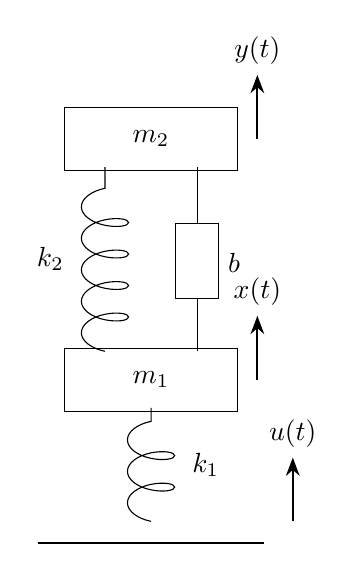
\begin{tikzpicture}[>=Stealth,scale=0.9]
  \draw[thick] (-1.6,-0.3)--(1.6,-0.3);
  \node[draw,minimum width=2.2cm,minimum height=0.8cm] (m1) at (0,2.0) {$m_1$};
  \node[draw,minimum width=2.2cm,minimum height=0.8cm] (m2) at (0,5.4) {$m_2$};

  \draw[decorate,decoration={coil,aspect=0.45,segment length=4mm,amplitude=3mm}]
    (0,0)--(0,1.6) node[midway,right=4mm]{$k_1$};

  \draw[decorate,decoration={coil,aspect=0.45,segment length=4mm,amplitude=3mm}]
    (-0.65,2.4)--(-0.65,5.0) node[midway,left=4mm]{$k_2$};

  \draw (0.65,2.4)--(0.65,3.15);
  \draw (0.35,3.15) rectangle (0.95,4.2);
  \draw (0.65,4.2)--(0.65,5.0);
  \node[right] at (0.95,3.65) {$b$};

  \draw[->,thick] (2.0,0)--(2.0,0.9) node[above]{$u(t)$};
  \draw[->,thick] (1.5,2.0)--(1.5,2.9) node[above]{$x(t)$};
  \draw[->,thick] (1.5,5.4)--(1.5,6.3) node[above]{$y(t)$};
\end{tikzpicture}
\end{center}

\loigiai
Phương trình động lực học của \(m_1\):
\[
m_1\ddot x
=
k_1(u-x)+k_2(y-x)+b(\dot y-\dot x).
\]
Suy ra
\[
m_1\ddot x+b(\dot x-\dot y)
+k_1(x-u)+k_2(x-y)=0. \tag{1}
\]
Với \(m_2\):
\[
m_2\ddot y
=
k_2(x-y)+b(\dot x-\dot y),
\]
hay
\[
m_2\ddot y+b(\dot y-\dot x)+k_2(y-x)=0. \tag{2}
\]
Lấy Laplace:
\[
[m_1s^2+bs+k_1+k_2]X-(bs+k_2)Y=k_1U,
\]
\[
-(bs+k_2)X+[m_2s^2+bs+k_2]Y=0.
\]
Giải hệ cho \(Y/U\):
\[
\boxed{
\frac{Y(s)}{U(s)}
=
\frac{k_1(bs+k_2)}
{
m_1m_2s^4+b(m_1+m_2)s^3
+[k_1m_2+k_2(m_1+m_2)]s^2
+bk_1s+k_1k_2
}.
}
\]

\textbf{A5 -- Không gian trạng thái}

\baitap{2.34}
\debai
(Nguồn A5.1) Với mạch \(L\) nối tiếp với nhánh \(R\parallel C\), đầu vào là \(v_i(t)\), đầu ra là \(v_C(t)\). Hãy lập mô hình không gian trạng thái.

\begin{center}
\begin{circuitikz}[european resistors,>=Stealth]
  \draw (0,0) node[ground]{} to[sV,l_=$v_i(t)$] (0,3)
        to[L=$L$,i>^=$i_L$] (3.2,3) node[circ] (n) {};
  \draw (n) to[R=$R$,i>_=$i_R$] (3.2,0) node[ground]{};
  \draw (n) -- (5.8,3) to[C=$C$,i>^=$i_C$,v^>=$v_C$] (5.8,0) node[ground]{};
\end{circuitikz}
\end{center}

\loigiai
Chọn
\[
x_1=v_C,\qquad x_2=i_L,\qquad u=v_i,\qquad y=v_C.
\]
KCL:
\[
i_L=\frac{v_C}{R}+C\dot v_C
\]
nên
\[
\dot x_1
=
-\frac1{RC}x_1+\frac1C x_2.
\]
KVL:
\[
v_i=L\dot i_L+v_C
\]
nên
\[
\dot x_2
=
-\frac1Lx_1+\frac1Lu.
\]
Do đó
\[
\boxed{
\dot x=
\begin{bmatrix}
-\dfrac1{RC}&\dfrac1C\\[2mm]
-\dfrac1L&0
\end{bmatrix}x
+
\begin{bmatrix}
0\\[1mm]\dfrac1L
\end{bmatrix}u,
\qquad
y=
\begin{bmatrix}1&0\end{bmatrix}x.
}
\]

\baitap{2.35}
\debai
(Nguồn A5.2) Với mạch \(R,L,C\) nối tiếp, đầu vào là \(v_i(t)\), đầu ra là điện áp tụ \(v_C(t)\). Hãy lập mô hình không gian trạng thái.

\begin{center}
\begin{circuitikz}[european resistors,>=Stealth]
  \draw (0,0) node[ground]{} to[sV,l_=$v_i(t)$] (0,3)
        to[R=$R$,i>^=$i(t)$] (2.5,3)
        to[L=$L$] (5.0,3)
        to[C=$C$,v^>=$v_C(t)$] (5.0,0) node[ground]{};
\end{circuitikz}
\end{center}

\loigiai
Chọn
\[
x_1=v_C,\qquad x_2=i,\qquad u=v_i,\qquad y=v_C.
\]
Với tụ:
\[
i=C\dot v_C
\quad\Rightarrow\quad
\dot x_1=\frac1C x_2.
\]
KVL:
\[
v_i=Ri+L\dot i+v_C,
\]
suy ra
\[
\dot x_2
=
-\frac1Lx_1-\frac RLx_2+\frac1Lu.
\]
Vậy
\[
\boxed{
\dot x=
\begin{bmatrix}
0&\dfrac1C\\[2mm]
-\dfrac1L&-\dfrac RL
\end{bmatrix}x
+
\begin{bmatrix}
0\\[1mm]\dfrac1L
\end{bmatrix}u,
\qquad
y=
\begin{bmatrix}1&0\end{bmatrix}x.
}
\]

\baitap{2.36}
\debai
(Nguồn A5.3) Lập mô hình không gian trạng thái của hệ hai khối lượng ở Bài 2.33, với đầu vào \(u(t)\) là chuyển vị nền và đầu ra \(y(t)\) là chuyển vị của \(m_2\).

\loigiai
Chọn
\[
x_1=x,\qquad
x_2=\dot x,\qquad
x_3=y,\qquad
x_4=\dot y.
\]
Từ các phương trình động lực học ở Bài 2.33:
\[
\dot x_1=x_2,
\]
\[
\dot x_2
=
-\frac{k_1+k_2}{m_1}x_1
-\frac b{m_1}x_2
+\frac{k_2}{m_1}x_3
+\frac b{m_1}x_4
+\frac{k_1}{m_1}u,
\]
\[
\dot x_3=x_4,
\]
\[
\dot x_4
=
\frac{k_2}{m_2}x_1
+\frac b{m_2}x_2
-\frac{k_2}{m_2}x_3
-\frac b{m_2}x_4.
\]
Do đó
\[
\boxed{
A=
\begin{bmatrix}
0&1&0&0\\
-\dfrac{k_1+k_2}{m_1}&-\dfrac b{m_1}&\dfrac{k_2}{m_1}&\dfrac b{m_1}\\
0&0&0&1\\
\dfrac{k_2}{m_2}&\dfrac b{m_2}&-\dfrac{k_2}{m_2}&-\dfrac b{m_2}
\end{bmatrix},
}
\]
\[
\boxed{
B=
\begin{bmatrix}
0\\[1mm]\dfrac{k_1}{m_1}\\[1mm]0\\[1mm]0
\end{bmatrix},
\qquad
C=
\begin{bmatrix}
0&0&1&0
\end{bmatrix},
\qquad D=0.
}
\]

\textbf{A6 -- Quan hệ giữa hàm truyền và không gian trạng thái}

\baitap{2.37}
\debai
(Nguồn A6.1) Tìm một mô hình không gian trạng thái của
\[
G(s)=\frac{Y(s)}{U(s)}
=
\frac{24}{s^3+9s^2+2s+6}.
\]

\loigiai
Từ
\[
(s^3+9s^2+2s+6)Y=24U
\]
suy ra
\[
y^{(3)}+9\ddot y+2\dot y+6y=24u.
\]
Chọn
\[
x_1=y,\qquad x_2=\dot y,\qquad x_3=\ddot y.
\]
Khi đó
\[
\boxed{
\dot x=
\begin{bmatrix}
0&1&0\\
0&0&1\\
-6&-2&-9
\end{bmatrix}x
+
\begin{bmatrix}
0\\0\\24
\end{bmatrix}u,
\qquad
y=
\begin{bmatrix}
1&0&0
\end{bmatrix}x.
}
\]

\baitap{2.38}
\debai
(Nguồn A6.2) Tìm một mô hình không gian trạng thái của
\[
G(s)=
\frac{2s+24}{s^3+6s^2+12s+16}.
\]

\loigiai
Dùng dạng chuẩn điều khiển:
\[
A=
\begin{bmatrix}
0&1&0\\
0&0&1\\
-16&-12&-6
\end{bmatrix},
\qquad
B=
\begin{bmatrix}
0\\0\\1
\end{bmatrix}.
\]
Với tử số
\[
2s+24=24+2s+0s^2,
\]
chọn
\[
C=
\begin{bmatrix}
24&2&0
\end{bmatrix},
\qquad D=0.
\]
Vậy
\[
\boxed{
\dot x=Ax+Bu,\qquad y=Cx,
}
\]
với các ma trận \(A,B,C\) ở trên.

\baitap{2.39}
\debai
(Nguồn A6.3) Tìm một mô hình không gian trạng thái của
\[
G(s)=
\frac{s^2+24s+2}
{2s^3+16s^2+12s+1}.
\]

\loigiai
Chuẩn hóa mẫu bằng cách chia cả tử và mẫu cho \(2\):
\[
G(s)
=
\frac{\frac12s^2+12s+1}
{s^3+8s^2+6s+\frac12}.
\]
Một dạng chuẩn điều khiển là
\[
\boxed{
A=
\begin{bmatrix}
0&1&0\\
0&0&1\\
-\frac12&-6&-8
\end{bmatrix},
\qquad
B=
\begin{bmatrix}
0\\0\\1
\end{bmatrix},
}
\]
\[
\boxed{
C=
\begin{bmatrix}
1&12&\frac12
\end{bmatrix},
\qquad D=0.
}
\]

\baitap{2.40}
\debai
(Nguồn A6.4) Cho
\[
\dot x=
\begin{bmatrix}
-5&-1\\
3&-1
\end{bmatrix}x
+
\begin{bmatrix}
2\\5
\end{bmatrix}u,
\qquad
y=
\begin{bmatrix}
1&2
\end{bmatrix}x.
\]
Tìm hàm truyền \(G(s)=Y(s)/U(s)\).

\loigiai
Dùng
\[
G(s)=C(sI-A)^{-1}B.
\]
Ta có
\[
sI-A=
\begin{bmatrix}
s+5&1\\
-3&s+1
\end{bmatrix},
\]
\[
\det(sI-A)
=
(s+5)(s+1)+3
=
s^2+6s+8
=
(s+2)(s+4),
\]
\[
\operatorname{adj}(sI-A)
=
\begin{bmatrix}
s+1&-1\\
3&s+5
\end{bmatrix}.
\]
Suy ra
\[
C\,\operatorname{adj}(sI-A)B
=
12s+59.
\]
Do đó
\[
\boxed{
G(s)=
\frac{12s+59}{(s+2)(s+4)}.
}
\]

\baitap{2.41}
\debai
(Nguồn A6.5) Cho
\[
\dot x=
\begin{bmatrix}
0&1&0\\
0&0&1\\
-1&-5&-7
\end{bmatrix}x
+
\begin{bmatrix}
2\\5\\0
\end{bmatrix}u,
\qquad
y=
\begin{bmatrix}
1&0&0
\end{bmatrix}x.
\]
Tìm hàm truyền \(G(s)\).

\loigiai
Ta có
\[
\det(sI-A)
=
s^3+7s^2+5s+1.
\]
Tính \(C(sI-A)^{-1}B\) cho tử số:
\[
2s^2+19s+45.
\]
Vì vậy
\[
\boxed{
G(s)=
\frac{2s^2+19s+45}
{s^3+7s^2+5s+1}
=
\frac{(s+5)(2s+9)}
{s^3+7s^2+5s+1}.
}
\]

\baitap{2.42}
\debai
(Nguồn A6.6) Hệ cơ gồm khối lượng \(m\), lò xo \(k\) và giảm chấn \(b\). Lực ngoài \(u(t)\) tác dụng theo chiều dương của chuyển vị \(y(t)\). Hãy:
\begin{itemize}
  \item lập mô hình không gian trạng thái;
  \item tìm hàm truyền \(Y(s)/U(s)\).
\end{itemize}

\begin{center}
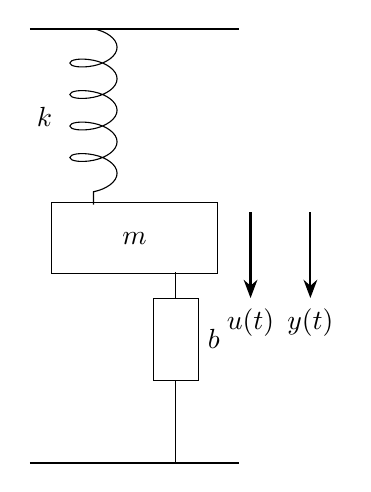
\begin{tikzpicture}[>=Stealth,scale=0.95]
  \draw[thick] (-1.4,5.8)--(1.4,5.8);
  \draw[thick] (-1.4,0)--(1.4,0);
  \node[draw,minimum width=2.1cm,minimum height=0.9cm] (m) at (0,3.0) {$m$};

  \draw[decorate,decoration={coil,aspect=0.45,segment length=4mm,amplitude=3mm}]
    (-0.55,5.8)--(-0.55,3.45) node[midway,left=4mm]{$k$};

  \draw (0.55,0)--(0.55,1.1);
  \draw (0.25,1.1) rectangle (0.85,2.2);
  \draw (0.55,2.2)--(0.55,2.55);
  \node[right] at (0.85,1.65) {$b$};

  \draw[->,thick] (1.55,3.35)--(1.55,2.2) node[below]{$u(t)$};
  \draw[->,thick] (2.35,3.35)--(2.35,2.2) node[below]{$y(t)$};
\end{tikzpicture}
\end{center}

\loigiai
Đo chuyển vị từ vị trí cân bằng tĩnh nên trọng lực đã được triệt bởi độ biến dạng cân bằng của lò xo. Phương trình động lực học:
\[
m\ddot y+b\dot y+ky=u.
\]
Chọn
\[
x_1=y,\qquad x_2=\dot y.
\]
Suy ra
\[
\boxed{
\dot x=
\begin{bmatrix}
0&1\\
-\dfrac km&-\dfrac bm
\end{bmatrix}x
+
\begin{bmatrix}
0\\[1mm]\dfrac1m
\end{bmatrix}u,
\qquad
y=
\begin{bmatrix}
1&0
\end{bmatrix}x.
}
\]
Lấy Laplace:
\[
(ms^2+bs+k)Y=U.
\]
Vậy
\[
\boxed{
\frac{Y(s)}{U(s)}
=
\frac1{ms^2+bs+k}.
}
\]


\clearpage
\chuong{3}{ĐẠI SỐ SƠ ĐỒ KHỐI VÀ GRAPH TÍN HIỆU}

\baitap{3.1}
\debai
Rút gọn sơ đồ khối sau và tìm hàm truyền kín \(G_k(s)=Y(s)/U(s)\). Sơ đồ dưới đây là dạng tương đương sau khi tách hai bộ tổng như trong ghi chép: tín hiệu \(U(s)\) đi qua \(G_1(s)\), đồng thời có một nhánh truyền thẳng \(U(s)\) cùng đi vào bộ tổng thứ nhất; bộ tổng thứ hai nhận hồi tiếp âm đơn vị từ \(Y(s)\), sau đó qua \(G_2(s)\).

\begin{center}
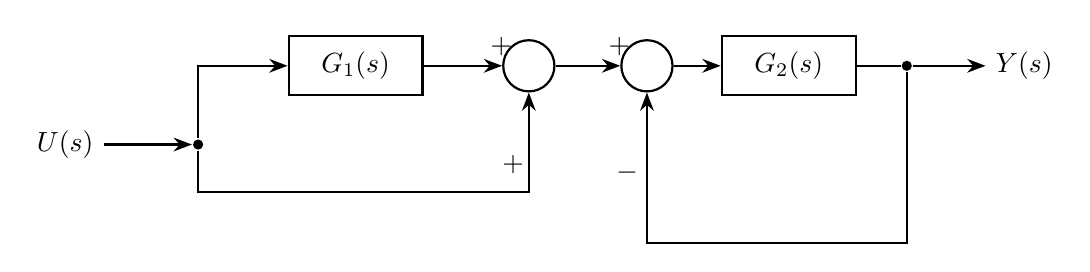
\begin{tikzpicture}[>=Stealth,thick]
  \node[pickoff] (p) at (0,0) {};
  \node[block] (g1) at (2,1.0) {$G_1(s)$};
  \node[sum] (s1) at (4.2,1.0) {};
  \node[sum] (s2) at (5.7,1.0) {};
  \node[block] (g2) at (7.5,1.0) {$G_2(s)$};
  \node[pickoff] (ypt) at (9.0,1.0) {};

  \draw[->] (-1.2,0) node[left]{$U(s)$} -- (p);
  \draw[->] (p) |- (g1.west);
  \draw[->] (g1.east) -- (s1.west);
  \draw[->] (p) -- (0,-0.6) -- (4.2,-0.6) -- (s1.south);
  \draw[->] (s1.east) -- (s2.west);
  \draw[->] (s2.east) -- (g2.west);
  \draw[->] (g2.east) -- (ypt) -- (10.0,1.0) node[right]{$Y(s)$};
  \draw[->] (ypt) -- (9.0,-1.25) -- (5.7,-1.25) -- (s2.south);

  \node at (3.85,1.25) {$+$};
  \node at (4.0,-0.25) {$+$};
  \node at (5.35,1.25) {$+$};
  \node at (5.45,-0.35) {$-$};
\end{tikzpicture}
\end{center}

\loigiai
Đầu ra của bộ tổng thứ nhất là
\[
X(s)=G_1(s)U(s)+U(s)
=\bigl[G_1(s)+1\bigr]U(s).
\]
Bộ \(G_2\) nằm trong vòng hồi tiếp âm đơn vị:
\[
Y(s)=G_2(s)\bigl[X(s)-Y(s)\bigr].
\]
Suy ra
\[
\bigl[1+G_2(s)\bigr]Y(s)
=G_2(s)X(s).
\]
Thay \(X(s)\):
\[
\boxed{
G_k(s)=\frac{Y(s)}{U(s)}
=
\frac{G_2(s)\bigl[G_1(s)+1\bigr]}
{1+G_2(s)}.}
\]

\baitap{3.2}
\debai
Rút gọn sơ đồ có \(G_2(s)\) và \(G_3(s)\) mắc song song sau \(G_1(s)\), toàn bộ nằm trong hồi tiếp âm đơn vị như hình. Tìm \(G_k(s)=Y(s)/U(s)\).

\begin{center}
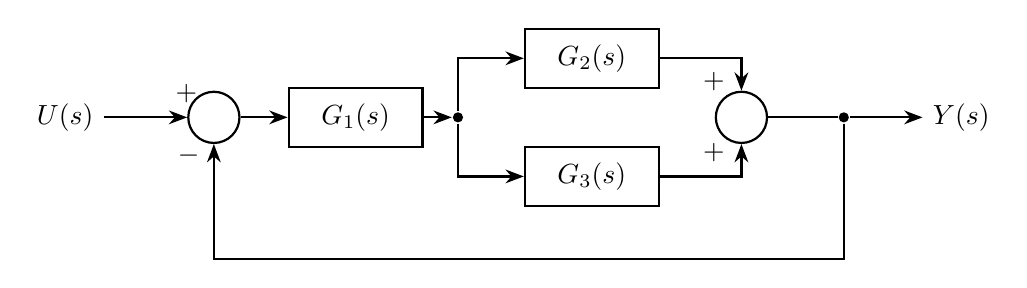
\begin{tikzpicture}[>=Stealth,thick]
  \node[sum] (s1) at (0,0) {};
  \node[block] (g1) at (1.8,0) {$G_1(s)$};
  \node[pickoff] (p) at (3.1,0) {};
  \node[block] (g2) at (4.8,0.75) {$G_2(s)$};
  \node[block] (g3) at (4.8,-0.75) {$G_3(s)$};
  \node[sum] (s2) at (6.7,0) {};
  \node[pickoff] (ypt) at (8.0,0) {};

  \draw[->] (-1.4,0) node[left]{$U(s)$} -- (s1.west);
  \draw[->] (s1.east) -- (g1.west);
  \draw[->] (g1.east) -- (p);
  \draw[->] (p) |- (g2.west);
  \draw[->] (p) |- (g3.west);
  \draw[->] (g2.east) -| (s2.north);
  \draw[->] (g3.east) -| (s2.south);
  \draw[->] (s2.east) -- (ypt) -- (9.0,0) node[right]{$Y(s)$};
  \draw[->] (ypt) -- (8.0,-1.8) -- (0,-1.8) -- (s1.south);

  \node at (-0.35,0.3) {$+$};
  \node at (-0.32,-0.48) {$-$};
  \node at (6.35,0.45) {$+$};
  \node at (6.35,-0.45) {$+$};
\end{tikzpicture}
\end{center}

\loigiai
Hai khối song song được gộp:
\[
G_{23}(s)=G_2(s)+G_3(s).
\]
Khâu truyền thuận trước khi đóng vòng là
\[
G_h(s)=G_1(s)\bigl[G_2(s)+G_3(s)\bigr].
\]
Do hồi tiếp âm đơn vị:
\[
\boxed{
G_k(s)
=
\frac{G_1(s)\bigl[G_2(s)+G_3(s)\bigr]}
{1+G_1(s)\bigl[G_2(s)+G_3(s)\bigr]}.}
\]

\baitap{3.3}
\debai
Trong bài biến đổi sơ đồ khối ở các trang 3--5 của ghi chép, sau khi chuyển bộ tổng, gộp các bộ tổng và chuyển điểm rẽ nhánh, sơ đồ được đưa về dạng tương đương dưới đây. Hãy tìm hàm truyền kín từ \(U(s)\) đến \(Y(s)\).

\begin{center}
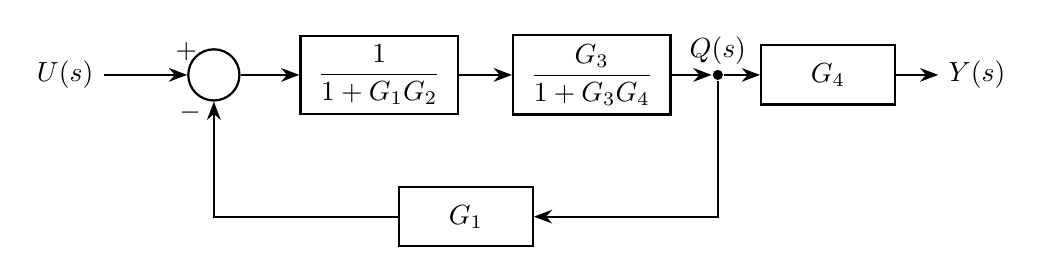
\begin{tikzpicture}[>=Stealth,thick]
  \node[sum] (s) at (0,0) {};
  \node[block,minimum width=2.0cm] (f1) at (2.1,0) {$\dfrac{1}{1+G_1G_2}$};
  \node[block,minimum width=2.0cm] (f2) at (4.8,0) {$\dfrac{G_3}{1+G_3G_4}$};
  \node[pickoff] (q) at (6.4,0) {};
  \node[block] (g4) at (7.8,0) {$G_4$};
  \node[block] (g1) at (3.2,-1.8) {$G_1$};

  \draw[->] (-1.4,0) node[left]{$U(s)$} -- (s.west);
  \draw[->] (s.east) -- (f1.west);
  \draw[->] (f1.east) -- (f2.west);
  \draw[->] (f2.east) -- (q);
  \draw[->] (q) -- (g4.west);
  \draw[->] (g4.east) -- (9.2,0) node[right]{$Y(s)$};
  \draw[->] (q) -- (6.4,-1.8) -- (g1.east);
  \draw[->] (g1.west) -- (0,-1.8) -- (s.south);

  \node at (-0.35,0.3) {$+$};
  \node at (-0.30,-0.48) {$-$};
  \node[above] at (q) {$Q(s)$};
\end{tikzpicture}
\end{center}

\loigiai
Đặt
\[
F_1(s)=\frac{1}{1+G_1G_2},
\qquad
F_2(s)=\frac{G_3}{1+G_3G_4}.
\]
Tại điểm rẽ trước \(G_4\):
\[
Q=F_1F_2\bigl(U-G_1Q\bigr).
\]
Do đó
\[
Q\bigl(1+G_1F_1F_2\bigr)=F_1F_2U.
\]
Suy ra
\[
\frac{Q}{U}
=
\frac{G_3}
{(1+G_1G_2)(1+G_3G_4)+G_1G_3}.
\]
Vì \(Y=G_4Q\):
\[
\boxed{
G_k(s)=\frac{Y}{U}
=
\frac{G_3G_4}
{(1+G_1G_2)(1+G_3G_4)+G_1G_3}.}
\]

\baitap{3.4}
\debai
Sau khi chuyển vị trí các bộ tổng trong ví dụ ở cuối trang 5 và đầu trang 6, sơ đồ tương đương có dạng như hình. Hãy tìm \(G(s)=C(s)/R(s)\).

\begin{center}
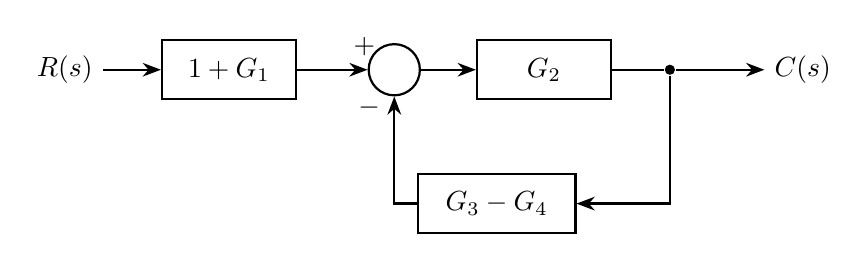
\begin{tikzpicture}[>=Stealth,thick]
  \node[block] (g1) at (0,0) {$1+G_1$};
  \node[sum] (s) at (2.1,0) {};
  \node[block] (g2) at (4.0,0) {$G_2$};
  \node[pickoff] (cpt) at (5.6,0) {};
  \node[block,minimum width=2.0cm] (fb) at (3.4,-1.7) {$G_3-G_4$};

  \draw[->] (-1.6,0) node[left]{$R(s)$} -- (g1.west);
  \draw[->] (g1.east) -- (s.west);
  \draw[->] (s.east) -- (g2.west);
  \draw[->] (g2.east) -- (cpt) -- (6.8,0) node[right]{$C(s)$};
  \draw[->] (cpt) -- (5.6,-1.7) -- (fb.east);
  \draw[->] (fb.west) -- (2.1,-1.7) -- (s.south);

  \node at (1.72,0.3) {$+$};
  \node at (1.78,-0.48) {$-$};
\end{tikzpicture}
\end{center}

\loigiai
Tín hiệu vào bộ tổng là
\[
(1+G_1)R-(G_3-G_4)C.
\]
Do đó
\[
C
=
G_2\Bigl[(1+G_1)R-(G_3-G_4)C\Bigr].
\]
Chuyển các số hạng chứa \(C\) về một phía:
\[
\Bigl[1+(G_3-G_4)G_2\Bigr]C
=(1+G_1)G_2R.
\]
Vậy
\[
\boxed{
G(s)=\frac{C(s)}{R(s)}
=
\frac{(1+G_1)G_2}
{1+(G_3-G_4)G_2}.}
\]

\baitap{3.5}
\debai
Cho hệ kín có khâu truyền thuận
\[
G(s)=\frac{10}{s(s+3)}
\]
và khâu hồi tiếp
\[
H(s)=\frac{1}{s+2},
\]
hồi tiếp âm như hình. Hãy:
\begin{itemize}
  \item tìm hàm truyền kín \(\bar G(s)=C(s)/R(s)\);
  \item xây dựng một mô hình không gian trạng thái liên tục của hệ kín.
\end{itemize}

\begin{center}
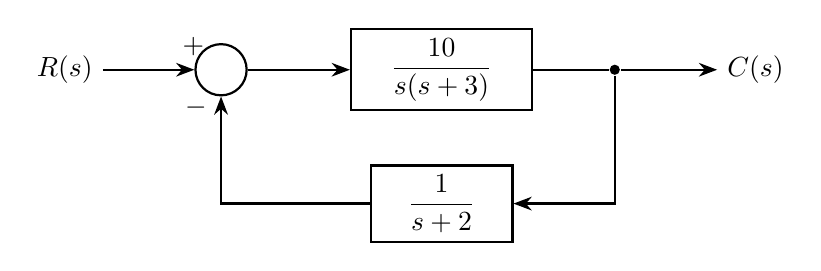
\begin{tikzpicture}[>=Stealth,thick]
  \node[sum] (s) at (0,0) {};
  \node[block,minimum width=2.3cm] (g) at (2.8,0) {$\dfrac{10}{s(s+3)}$};
  \node[pickoff] (cpt) at (5.0,0) {};
  \node[block,minimum width=1.8cm] (h) at (2.8,-1.7) {$\dfrac{1}{s+2}$};

  \draw[->] (-1.5,0) node[left]{$R(s)$} -- (s.west);
  \draw[->] (s.east) -- (g.west);
  \draw[->] (g.east) -- (cpt) -- (6.3,0) node[right]{$C(s)$};
  \draw[->] (cpt) -- (5.0,-1.7) -- (h.east);
  \draw[->] (h.west) -- (0,-1.7) -- (s.south);

  \node at (-0.35,0.3) {$+$};
  \node at (-0.32,-0.48) {$-$};
\end{tikzpicture}
\end{center}

\loigiai
Với hồi tiếp âm:
\[
\bar G(s)
=
\frac{G(s)}{1+G(s)H(s)}.
\]
Thay \(G,H\):
\[
\bar G(s)
=
\frac{\dfrac{10}{s(s+3)}}
{1+\dfrac{10}{s(s+3)}\dfrac{1}{s+2}}
=
\frac{10(s+2)}
{s(s+3)(s+2)+10}.
\]
Khai triển mẫu:
\[
s(s+3)(s+2)+10
=s^3+5s^2+6s+10.
\]
Do đó
\[
\boxed{
\bar G(s)
=
\frac{10s+20}
{s^3+5s^2+6s+10}.}
\]

Từ
\[
\bigl(s^3+5s^2+6s+10\bigr)C(s)
=
(10s+20)R(s),
\]
với điều kiện đầu bằng không:
\[
c^{(3)}+5\ddot c+6\dot c+10c
=
10\dot r+20r. \tag{1}
\]

Theo cách chọn biến trạng thái trong ghi chép, đặt
\[
x_1=c,
\]
\[
x_2=\dot x_1-\beta_1r
=\dot c-\beta_1r,
\]
\[
x_3=\dot x_2-\beta_2r
=\ddot c-\beta_1\dot r-\beta_2r.
\]
Khi đó
\[
\dot x_1=x_2+\beta_1r,
\qquad
\dot x_2=x_3+\beta_2r.
\]
Đặt thêm hệ số \(\beta_3\) để viết
\[
\dot x_3
=-10x_1-6x_2-5x_3+\beta_3r.
\]
Khi quy đổi ngược về phương trình của \(c(t)\), vế phải có dạng
\[
\beta_1\ddot r
+(5\beta_1+\beta_2)\dot r
+(6\beta_1+5\beta_2+\beta_3)r.
\]
So sánh với vế phải \(10\dot r+20r\) của (1):
\[
\beta_1=0,
\]
\[
5\beta_1+\beta_2=10
\quad\Rightarrow\quad
\beta_2=10,
\]
\[
6\beta_1+5\beta_2+\beta_3=20
\quad\Rightarrow\quad
\beta_3=-30.
\]
Vì vậy
\[
\dot x_1=x_2,
\]
\[
\dot x_2=x_3+10r,
\]
\[
\dot x_3=-10x_1-6x_2-5x_3-30r.
\]
Mô hình trạng thái là
\[
\boxed{
\begin{bmatrix}
\dot x_1\\
\dot x_2\\
\dot x_3
\end{bmatrix}
=
\begin{bmatrix}
0&1&0\\
0&0&1\\
-10&-6&-5
\end{bmatrix}
\begin{bmatrix}
x_1\\
x_2\\
x_3
\end{bmatrix}
+
\begin{bmatrix}
0\\
10\\
-30
\end{bmatrix}r
}
\]
và vì \(c=x_1\),
\[
\boxed{
c=
\begin{bmatrix}
1&0&0
\end{bmatrix}x,
\qquad D=0.}
\]


\baitap{3.6}
\debai
Chuyển hai sơ đồ khối cơ bản sau sang graph tín hiệu và xác định quan hệ vào--ra.

\textbf{a) Hai nhánh song song cùng đi vào một bộ tổng dương.}

\begin{center}
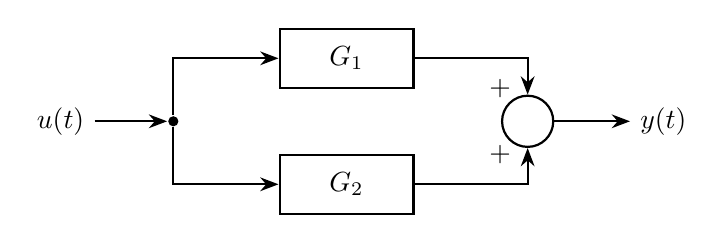
\begin{tikzpicture}[>=Stealth,thick]
  \node[pickoff] (u) at (0,0) {};
  \node[block] (g1) at (2.2,0.8) {$G_1$};
  \node[block] (g2) at (2.2,-0.8) {$G_2$};
  \node[sum] (sum) at (4.5,0) {};
  \draw[->] (-1.0,0) node[left]{$u(t)$} -- (u);
  \draw[->] (u) |- (g1.west);
  \draw[->] (u) |- (g2.west);
  \draw[->] (g1.east) -| (sum.north);
  \draw[->] (g2.east) -| (sum.south);
  \draw[->] (sum.east) -- (5.8,0) node[right]{$y(t)$};
  \node at (4.15,0.42) {$+$};
  \node at (4.15,-0.42) {$+$};
\end{tikzpicture}
\qquad
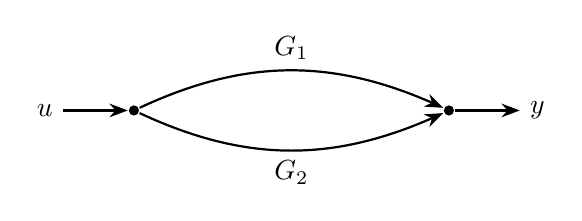
\begin{tikzpicture}[>=Stealth,thick]
  \node[pickoff] (u) at (0,0) {};
  \node[pickoff] (y) at (4.0,0) {};
  \draw[->] (-0.9,0) node[left]{$u$} -- (u);
  \draw[->] (u) to[bend left=25] node[above]{$G_1$} (y);
  \draw[->] (u) to[bend right=25] node[below]{$G_2$} (y);
  \draw[->] (y) -- (4.9,0) node[right]{$y$};
\end{tikzpicture}
\end{center}

\textbf{b) Một khâu thuận \(G_1\) với hồi tiếp âm \(G_2\) tại bộ tổng.}

\begin{center}
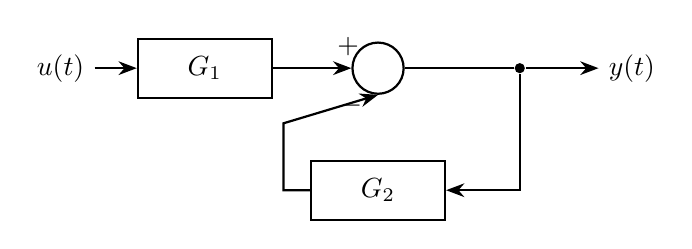
\begin{tikzpicture}[>=Stealth,thick]
  \node[block] (g1) at (0,0) {$G_1$};
  \node[sum] (sum) at (2.2,0) {};
  \node[pickoff] (ypt) at (4.0,0) {};
  \node[block] (g2) at (2.2,-1.55) {$G_2$};
  \draw[->] (-1.4,0) node[left]{$u(t)$} -- (g1.west);
  \draw[->] (g1.east) -- (sum.west);
  \draw[->] (sum.east) -- (ypt) -- (5.0,0) node[right]{$y(t)$};
  \draw[->] (ypt) -- (4.0,-1.55) -- (g2.east);
  \draw[->] (g2.west) -- (1.0,-1.55) -- (1.0,-0.7) -- (sum.south);
  \node at (1.82,0.28) {$+$};
  \node at (1.86,-0.48) {$-$};
\end{tikzpicture}
\qquad
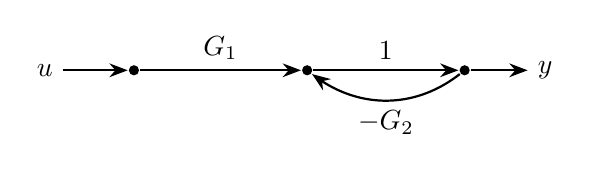
\begin{tikzpicture}[>=Stealth,thick]
  \node[pickoff] (u) at (0,0) {};
  \node[pickoff] (x) at (2.2,0) {};
  \node[pickoff] (y) at (4.2,0) {};
  \draw[->] (-0.9,0) node[left]{$u$} -- (u);
  \draw[->] (u) -- node[above]{$G_1$} (x);
  \draw[->] (x) -- node[above]{$1$} (y);
  \draw[->] (y) -- (5.0,0) node[right]{$y$};
  \draw[->] (y) to[bend left=38] node[below]{$-G_2$} (x);
\end{tikzpicture}
\end{center}

\loigiai
Trong graph tín hiệu:
\begin{itemize}
  \item mỗi nút biểu diễn một tín hiệu;
  \item mỗi nhánh có hướng và mang một hệ số truyền;
  \item tín hiệu tại một nút bằng tổng các tín hiệu đi vào nút đó sau khi nhân với hệ số truyền của từng nhánh.
\end{itemize}

Với câu a:
\[
y=G_1u+G_2u,
\]
nên
\[
\boxed{\frac{Y}{U}=G_1+G_2.}
\]

Với câu b, gọi tín hiệu ngay sau bộ tổng là \(x\). Từ graph:
\[
x=G_1u-G_2y,
\qquad
y=x.
\]
Do đó
\[
y=G_1u-G_2y
\]
và
\[
\boxed{
\frac{Y}{U}
=
\frac{G_1}{1+G_2}.}
\]

\baitap{3.7}
\debai
Cho graph tín hiệu dưới đây. Dùng công thức Mason để tìm hàm truyền tổng
\[
G(s)=\frac{C(s)}{R(s)}.
\]

\begin{center}
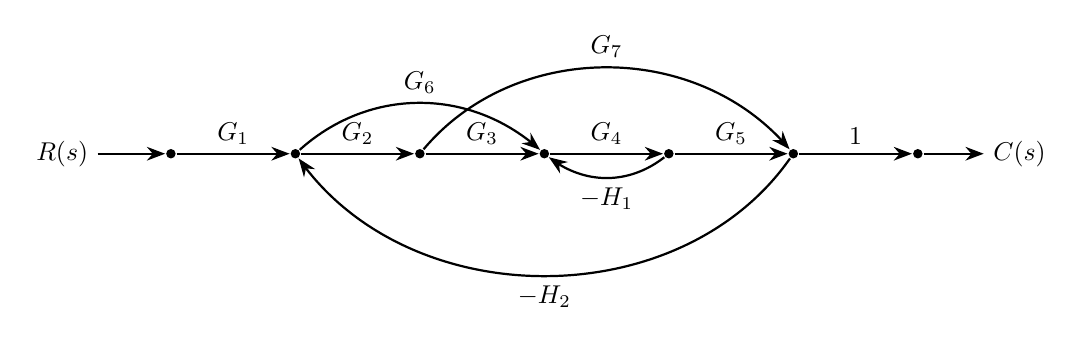
\begin{tikzpicture}[>=Stealth,thick,scale=0.93,transform shape]
  \node[pickoff] (n0) at (0,0) {};
  \node[pickoff] (n1) at (1.7,0) {};
  \node[pickoff] (n2) at (3.4,0) {};
  \node[pickoff] (n3) at (5.1,0) {};
  \node[pickoff] (n4) at (6.8,0) {};
  \node[pickoff] (n5) at (8.5,0) {};
  \node[pickoff] (n6) at (10.2,0) {};

  \draw[->] (-1.0,0) node[left]{$R(s)$} -- (n0);
  \draw[->] (n0) -- node[above]{$G_1$} (n1);
  \draw[->] (n1) -- node[above]{$G_2$} (n2);
  \draw[->] (n2) -- node[above]{$G_3$} (n3);
  \draw[->] (n3) -- node[above]{$G_4$} (n4);
  \draw[->] (n4) -- node[above]{$G_5$} (n5);
  \draw[->] (n5) -- node[above]{$1$} (n6);
  \draw[->] (n6) -- (11.1,0) node[right]{$C(s)$};

  \draw[->] (n1) to[bend left=42] node[above]{$G_6$} (n3);
  \draw[->] (n2) to[bend left=50] node[above]{$G_7$} (n5);

  \draw[->] (n4) to[bend left=38] node[below]{$-H_1$} (n3);
  \draw[->] (n5) to[bend left=55] node[below]{$-H_2$} (n1);
\end{tikzpicture}
\end{center}

\loigiai
Công thức Mason:
\[
\boxed{
G(s)=\frac{1}{\Delta}\sum_k P_k\Delta_k
}
\]
với
\[
\Delta
=
1-\sum L_i
+\sum L_iL_j
-\sum L_iL_jL_m+\cdots,
\]
trong đó chỉ lấy tích của các vòng lặp không chạm nhau.

\textbf{Bước 1: các đường truyền thuận.}
Từ graph có ba đường truyền thuận:
\[
P_1=G_1G_2G_3G_4G_5,
\]
\[
P_2=G_1G_6G_4G_5,
\]
\[
P_3=G_1G_2G_7.
\]

\textbf{Bước 2: các vòng lặp.}
Các vòng lặp là
\[
L_1=-G_4H_1,
\]
\[
L_2=-G_2G_3G_4G_5H_2,
\]
\[
L_3=-G_6G_4G_5H_2,
\]
\[
L_4=-G_2G_7H_2.
\]
Trong bốn vòng trên, chỉ có \(L_1\) và \(L_4\) không chạm nhau. Vì vậy
\[
\boxed{
\Delta
=
1-(L_1+L_2+L_3+L_4)+L_1L_4.
}
\]

\textbf{Bước 3: xác định \(\Delta_k\).}
Đường \(P_1\) chạm tất cả các vòng lặp:
\[
\Delta_1=1.
\]
Đường \(P_2\) cũng chạm tất cả các vòng lặp:
\[
\Delta_2=1.
\]
Với \(P_3\), chỉ có vòng \(L_1\) không chạm \(P_3\):
\[
\Delta_3=1-L_1.
\]

\textbf{Bước 4: áp dụng công thức Mason.}
\[
\boxed{
G(s)
=
\frac{
P_1+P_2+P_3(1-L_1)
}{
1-(L_1+L_2+L_3+L_4)+L_1L_4
}.}
\]
Thay trực tiếp các \(P_k,L_i\):
\[
\boxed{
G(s)=
\frac{
G_1G_2G_3G_4G_5
+G_1G_6G_4G_5
+G_1G_2G_7(1+G_4H_1)
}{
\Delta
}
}
\]
với
\[
\Delta=
1+G_4H_1
+G_2G_3G_4G_5H_2
+G_6G_4G_5H_2
+G_2G_7H_2
+G_2G_4G_7H_1H_2.
\]

\baitap{3.8}
\debai
Cho graph tín hiệu sau. Dùng công thức Mason để tìm
\[
G(s)=\frac{Y(s)}{U(s)}.
\]

\begin{center}
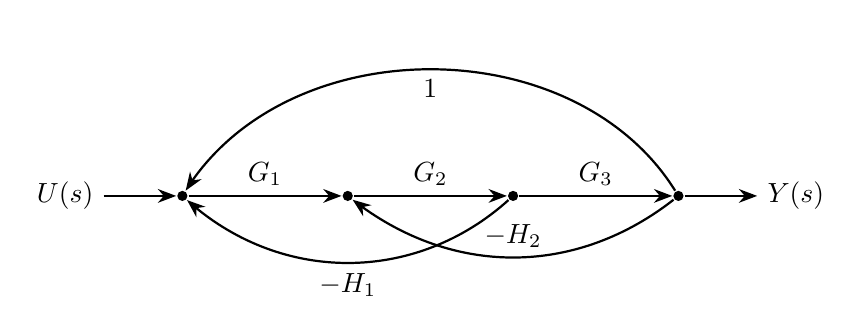
\begin{tikzpicture}[>=Stealth,thick,scale=1.0,transform shape]
  \node[pickoff] (n0) at (0,0) {};
  \node[pickoff] (n1) at (2.1,0) {};
  \node[pickoff] (n2) at (4.2,0) {};
  \node[pickoff] (n3) at (6.3,0) {};

  \draw[->] (-1.0,0) node[left]{$U(s)$} -- (n0);
  \draw[->] (n0) -- node[above]{$G_1$} (n1);
  \draw[->] (n1) -- node[above]{$G_2$} (n2);
  \draw[->] (n2) -- node[above]{$G_3$} (n3);
  \draw[->] (n3) -- (7.3,0) node[right]{$Y(s)$};

  \draw[->] (n2) to[bend left=42] node[below]{$-H_1$} (n0);
  \draw[->] (n3) to[bend left=38] node[above]{$-H_2$} (n1);
  \draw[->] (n3) to[bend right=58] node[below]{$1$} (n0);
\end{tikzpicture}
\end{center}

\loigiai
Có một đường truyền thuận
\[
P_1=G_1G_2G_3,
\]
và ba vòng lặp
\[
L_1=-G_1G_2H_1,\qquad
L_2=-G_2G_3H_2,\qquad
L_3=G_1G_2G_3.
\]
Ba vòng lặp đều chạm nhau nên không có tích của các vòng không chạm nhau:
\[
\Delta=1-(L_1+L_2+L_3).
\]
Mọi vòng lặp đều chạm đường thuận \(P_1\), do đó \(\Delta_1=1\). Theo Mason:
\[
\boxed{
G(s)=\frac{P_1\Delta_1}{\Delta}
=
\frac{G_1G_2G_3}
{1+G_1G_2H_1+G_2G_3H_2-G_1G_2G_3}.}
\]




\subsection*{Bài tập bổ sung từ bộ đề A7 -- Sơ đồ khối}

\baitap{3.9}
\debai
(Nguồn A7.1) Rút gọn sơ đồ khối và tìm
\[
\frac{C(s)}{R(s)}.
\]

\begin{center}
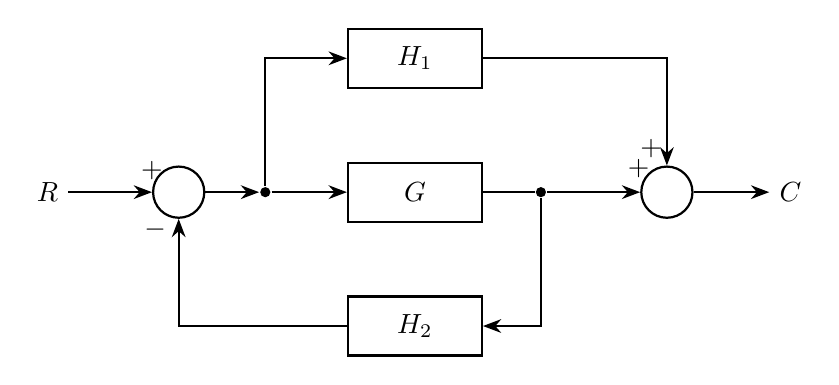
\begin{tikzpicture}[>=Stealth,thick]
  \node[sum] (s1) at (0,0) {};
  \node[pickoff] (e) at (1.1,0) {};
  \node[block] (g) at (3.0,0) {$G$};
  \node[pickoff] (gp) at (4.6,0) {};
  \node[sum] (s2) at (6.2,0) {};
  \node[block] (h1) at (3.0,1.7) {$H_1$};
  \node[block] (h2) at (3.0,-1.7) {$H_2$};

  \draw[->] (-1.4,0) node[left]{$R$} -- (s1.west);
  \draw[->] (s1.east) -- (e);
  \draw[->] (e) -- (g.west);
  \draw[->] (e) |- (h1.west);
  \draw[->] (g.east) -- (gp) -- (s2.west);
  \draw[->] (h1.east) -| (s2.north);
  \draw[->] (s2.east) -- (7.5,0) node[right]{$C$};
  \draw[->] (gp) |- (h2.east);
  \draw[->] (h2.west) -- (0,-1.7) -- (s1.south);

  \node at (-0.34,0.28) {$+$};
  \node at (-0.30,-0.48) {$-$};
  \node at (5.84,0.30) {$+$};
  \node at (6.0,0.55) {$+$};
\end{tikzpicture}
\end{center}

\loigiai
Gọi tín hiệu sau bộ tổng thứ nhất là \(E\). Nhánh hồi tiếp lấy sau khối \(G\):
\[
E=R-H_2GE.
\]
Do đó
\[
E=\frac{R}{1+GH_2}.
\]
Bộ tổng đầu ra cộng hai nhánh \(GE\) và \(H_1E\):
\[
C=(G+H_1)E.
\]
Suy ra
\[
\boxed{
\frac{C}{R}
=
\frac{G+H_1}{1+GH_2}.
}
\]

\baitap{3.10}
\debai
(Nguồn A7.2) Rút gọn sơ đồ khối sau và tìm \(C(s)/R(s)\).

\begin{center}
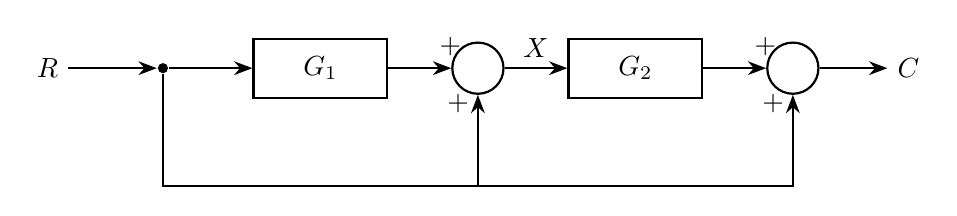
\begin{tikzpicture}[>=Stealth,thick]
  \node[pickoff] (r) at (0,0) {};
  \node[block] (g1) at (2,0) {$G_1$};
  \node[sum] (s1) at (4,0) {};
  \node[block] (g2) at (6,0) {$G_2$};
  \node[sum] (s2) at (8,0) {};
  \draw[->] (-1.2,0) node[left]{$R$}--(r);
  \draw[->] (r)--(g1.west);
  \draw[->] (g1.east)--(s1.west);
  \draw[->] (s1.east)--node[above]{$X$}(g2.west);
  \draw[->] (g2.east)--(s2.west);
  \draw[->] (s2.east)--(9.2,0) node[right]{$C$};
  \draw[->] (r)--(0,-1.5)--(4,-1.5)--(s1.south);
  \draw[->] (4,-1.5)--(8,-1.5)--(s2.south);
  \node at (3.65,0.28) {$+$};
  \node at (3.75,-0.45) {$+$};
  \node at (7.65,0.28) {$+$};
  \node at (7.75,-0.45) {$+$};
\end{tikzpicture}
\end{center}

\loigiai
Tại bộ tổng thứ nhất:
\[
X=(G_1+1)R.
\]
Tại bộ tổng thứ hai:
\[
C=G_2X+R.
\]
Do đó
\[
\boxed{
\frac{C}{R}
=
G_2(G_1+1)+1.
}
\]

\baitap{3.11}
\debai
(Nguồn A7.3) Với sơ đồ khối sau, tìm \(Y(s)/U(s)\).

\begin{center}
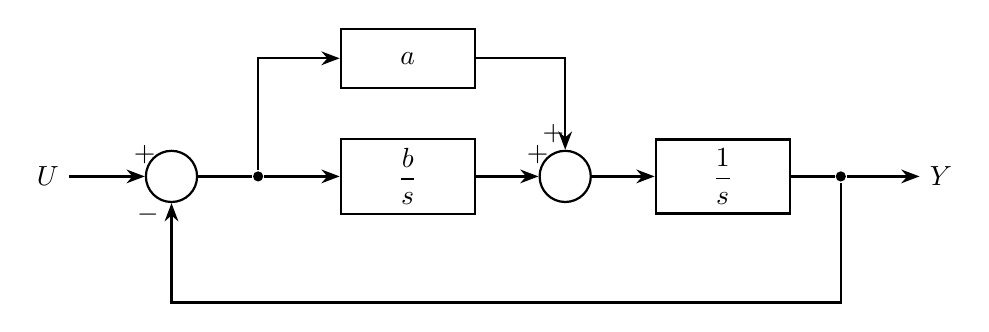
\begin{tikzpicture}[>=Stealth,thick]
  \node[sum] (s1) at (0,0) {};
  \node[pickoff] (e) at (1.1,0) {};
  \node[block] (bs) at (3.0,0) {$\dfrac{b}{s}$};
  \node[block] (a) at (3.0,1.5) {$a$};
  \node[sum] (s2) at (5.0,0) {};
  \node[block] (int) at (7.0,0) {$\dfrac1s$};
  \node[pickoff] (y) at (8.5,0) {};
  \draw[->] (-1.3,0) node[left]{$U$}--(s1.west);
  \draw[->] (s1.east)--(e)--(bs.west);
  \draw[->] (e)|-(a.west);
  \draw[->] (bs.east)--(s2.west);
  \draw[->] (a.east)-|(s2.north);
  \draw[->] (s2.east)--(int.west);
  \draw[->] (int.east)--(y)--(9.5,0) node[right]{$Y$};
  \draw[->] (y)--(8.5,-1.6)--(0,-1.6)--(s1.south);
  \node at (-0.34,0.28) {$+$};
  \node at (-0.30,-0.48) {$-$};
  \node at (4.65,0.28) {$+$};
  \node at (4.85,0.55) {$+$};
\end{tikzpicture}
\end{center}

\loigiai
Khâu truyền thuận từ sai lệch \(E\) đến \(Y\) là
\[
F(s)
=
\left(a+\frac bs\right)\frac1s
=
\frac{as+b}{s^2}.
\]
Hệ hồi tiếp âm đơn vị nên
\[
\frac{Y}{U}
=
\frac{F}{1+F}.
\]
Vì vậy
\[
\boxed{
\frac{Y(s)}{U(s)}
=
\frac{as+b}{s^2+as+b}.
}
\]

\baitap{3.12}
\debai
(Nguồn A7.4) Rút gọn sơ đồ và tìm \(C(s)/R(s)\).

\begin{center}
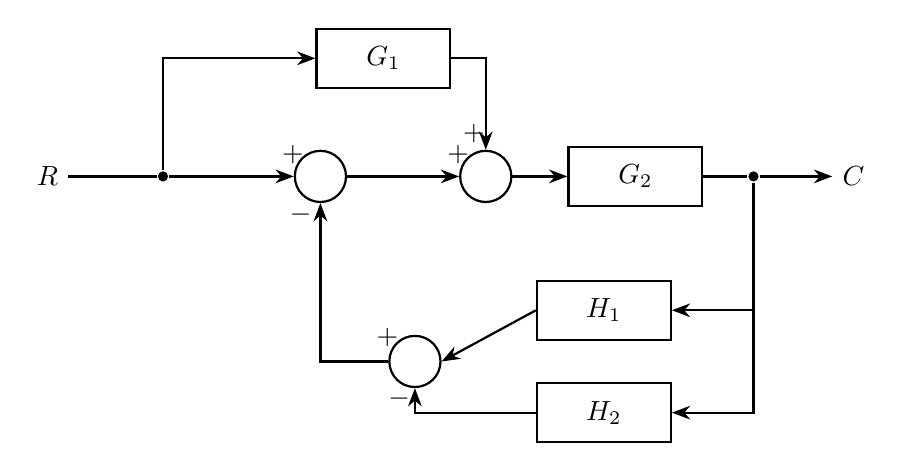
\begin{tikzpicture}[>=Stealth,thick]
  \node[pickoff] (r) at (0,0) {};
  \node[sum] (s1) at (2,0) {};
  \node[sum] (s2) at (4.1,0) {};
  \node[block] (g2) at (6,0) {$G_2$};
  \node[pickoff] (c) at (7.5,0) {};
  \node[block] (g1) at (2.8,1.5) {$G_1$};
  \node[block] (h1) at (5.6,-1.7) {$H_1$};
  \node[block] (h2) at (5.6,-3.0) {$H_2$};
  \node[sum] (sf) at (3.2,-2.35) {};

  \draw[->] (-1.2,0) node[left]{$R$}--(r)--(s1.west);
  \draw[->] (r)|-(g1.west);
  \draw[->] (s1.east)--(s2.west);
  \draw[->] (g1.east)-|(s2.north);
  \draw[->] (s2.east)--(g2.west);
  \draw[->] (g2.east)--(c)--(8.5,0) node[right]{$C$};

  \draw[->] (c)--(7.5,-1.7)--(h1.east);
  \draw[->] (c)--(7.5,-3.0)--(h2.east);
  \draw[->] (h1.west)--(sf.east);
  \draw[->] (h2.west)-|(sf.south);
  \draw[->] (sf.west)--(2,-2.35)--(s1.south);

  \node at (1.65,0.28) {$+$};
  \node at (1.75,-0.48) {$-$};
  \node at (3.75,0.28) {$+$};
  \node at (3.95,0.55) {$+$};
  \node at (2.85,-2.05) {$+$};
  \node at (3.0,-2.82) {$-$};
\end{tikzpicture}
\end{center}

\loigiai
Bộ tổng hồi tiếp phía dưới tạo
\[
F_b=(H_1-H_2)C.
\]
Tại bộ tổng thứ nhất:
\[
E=R-(H_1-H_2)C.
\]
Bộ tổng thứ hai nhận \(E\) và \(G_1R\):
\[
C=G_2(E+G_1R).
\]
Suy ra
\[
C
=
G_2[(1+G_1)R-(H_1-H_2)C].
\]
Do đó
\[
\boxed{
\frac{C}{R}
=
\frac{(1+G_1)G_2}
{1+G_2(H_1-H_2)}.
}
\]

\baitap{3.13}
\debai
(Nguồn A7.5) Rút gọn sơ đồ và tìm \(C(s)/R(s)\).

\begin{center}
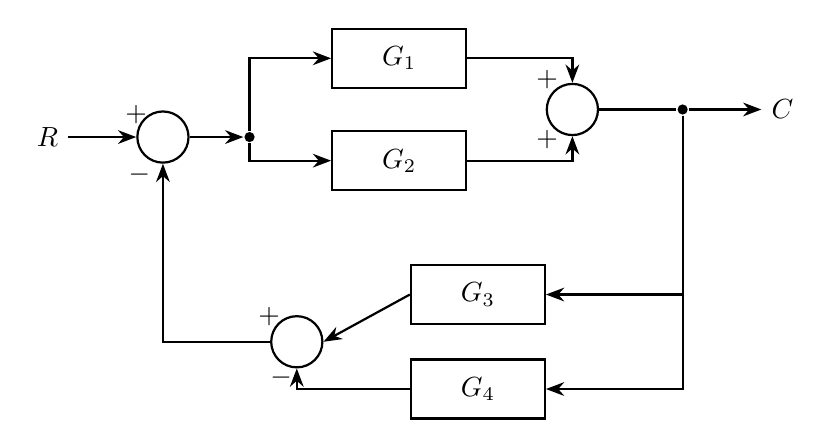
\begin{tikzpicture}[>=Stealth,thick]
  \node[sum] (s1) at (0,0) {};
  \node[pickoff] (e) at (1.1,0) {};
  \node[block] (g1) at (3,1.0) {$G_1$};
  \node[block] (g2) at (3,-0.3) {$G_2$};
  \node[sum] (s2) at (5.2,0.35) {};
  \node[pickoff] (c) at (6.6,0.35) {};
  \node[block] (g3) at (4.0,-2.0) {$G_3$};
  \node[block] (g4) at (4.0,-3.2) {$G_4$};
  \node[sum] (sf) at (1.7,-2.6) {};

  \draw[->] (-1.2,0) node[left]{$R$}--(s1.west);
  \draw[->] (s1.east)--(e);
  \draw[->] (e)|-(g1.west);
  \draw[->] (e)|-(g2.west);
  \draw[->] (g1.east)-|(s2.north);
  \draw[->] (g2.east)-|(s2.south);
  \draw[->] (s2.east)--(c)--(7.6,0.35) node[right]{$C$};

  \draw[->] (c)--(6.6,-2.0)--(g3.east);
  \draw[->] (c)--(6.6,-3.2)--(g4.east);
  \draw[->] (g3.west)--(sf.east);
  \draw[->] (g4.west)-|(sf.south);
  \draw[->] (sf.west)--(0,-2.6)--(s1.south);

  \node at (-0.34,0.28) {$+$};
  \node at (-0.30,-0.48) {$-$};
  \node at (4.88,0.73) {$+$};
  \node at (4.88,-0.03) {$+$};
  \node at (1.35,-2.28) {$+$};
  \node at (1.50,-3.06) {$-$};
\end{tikzpicture}
\end{center}

\loigiai
Hai khối thuận song song:
\[
G_f=G_1+G_2.
\]
Nhánh hồi tiếp phía dưới:
\[
H=G_3-G_4.
\]
Với hồi tiếp âm:
\[
C=G_f(R-HC).
\]
Suy ra
\[
\boxed{
\frac{C}{R}
=
\frac{G_1+G_2}
{1+(G_1+G_2)(G_3-G_4)}.
}
\]

\baitap{3.14}
\debai
(Nguồn A7.6) Hệ có bộ điều khiển
\[
G_c(s)=\frac1s,
\]
đối tượng
\[
G_p(s)=\frac{10}{s+5},
\]
và cảm biến
\[
H(s)=\frac1{s+1}.
\]
Hồi tiếp âm. Tìm hàm truyền kín \(Y(s)/U(s)\).

\begin{center}
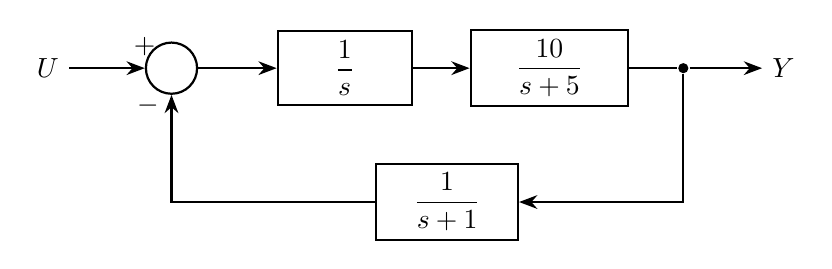
\begin{tikzpicture}[>=Stealth,thick]
  \node[sum] (s1) at (0,0) {};
  \node[block] (gc) at (2.2,0) {$\dfrac1s$};
  \node[block,minimum width=2cm] (gp) at (4.8,0) {$\dfrac{10}{s+5}$};
  \node[pickoff] (y) at (6.5,0) {};
  \node[block,minimum width=1.8cm] (h) at (3.5,-1.7) {$\dfrac1{s+1}$};

  \draw[->] (-1.3,0) node[left]{$U$}--(s1.west);
  \draw[->] (s1.east)--(gc.west);
  \draw[->] (gc.east)--(gp.west);
  \draw[->] (gp.east)--(y)--(7.5,0) node[right]{$Y$};
  \draw[->] (y)--(6.5,-1.7)--(h.east);
  \draw[->] (h.west)--(0,-1.7)--(s1.south);

  \node at (-0.34,0.28) {$+$};
  \node at (-0.30,-0.48) {$-$};
\end{tikzpicture}
\end{center}

\loigiai
Khâu truyền thuận:
\[
G(s)=G_cG_p
=
\frac{10}{s(s+5)}.
\]
Với hồi tiếp âm không đơn vị:
\[
\frac{Y}{U}
=
\frac{G}{1+GH}.
\]
Suy ra
\[
\frac{Y}{U}
=
\frac{\dfrac{10}{s(s+5)}}
{1+\dfrac{10}{s(s+5)(s+1)}}.
\]
Rút gọn:
\[
\boxed{
\frac{Y(s)}{U(s)}
=
\frac{10(s+1)}
{s(s+5)(s+1)+10}
=
\frac{10(s+1)}
{s^3+6s^2+5s+10}.
}
\]


\chuong{4}{ĐẶC TÍNH ĐỘNG HỌC VÀ ĐÁP ỨNG TẦN SỐ}

\baitap{4.1}
\debai
Cho hệ có hàm truyền
\[
G(s)=\frac{s+1}{s(s+5)}.
\]
Hãy:
\begin{itemize}
  \item tìm đáp ứng xung \(g(t)\);
  \item tìm đáp ứng của hệ khi tín hiệu vào là \(r(t)=2\,1(t)\).
\end{itemize}

\loigiai
Theo định nghĩa, đáp ứng xung là
\[
g(t)=\Lap^{-1}\{G(s)\}.
\]
Tách phân thức:
\[
\frac{s+1}{s(s+5)}
=
\frac{1/5}{s}+\frac{4/5}{s+5}.
\]
Vì vậy
\[
\boxed{
g(t)=
\left(\frac15+\frac45e^{-5t}\right)1(t).
}
\]

Với
\[
r(t)=2\,1(t)
\quad\Longrightarrow\quad
R(s)=\frac2s,
\]
đầu ra trong miền Laplace là
\[
C(s)=G(s)R(s)
=
\frac{2(s+1)}{s^2(s+5)}.
\]
Tách phân thức:
\[
C(s)
=
\frac{8}{25}\frac1s
+\frac25\frac1{s^2}
-\frac{8}{25}\frac1{s+5}.
\]
Do đó
\[
\boxed{
c(t)=
\left(
\frac{8}{25}
+\frac25t
-\frac{8}{25}e^{-5t}
\right)1(t).
}
\]
Dấu của số hạng \(e^{-5t}\) là âm, phù hợp với hệ số
\(-8/25\) trong phép tách phân thức và cho \(c(0)=0\).

\baitap{4.2}
\debai
Biết đáp ứng bước đơn vị của một hệ là
\[
h(t)=\left(1-3e^{-2t}+2e^{-3t}\right)1(t).
\]
Hãy tìm hàm truyền \(G(s)\).

\loigiai
Với hệ tuyến tính bất biến theo thời gian, đáp ứng xung là đạo hàm của đáp ứng bước:
\[
g(t)=\frac{dh(t)}{dt}.
\]
Do
\[
h(0^+)=1-3+2=0,
\]
không xuất hiện thành phần xung Dirac khi lấy đạo hàm. Vì vậy
\[
g(t)=6e^{-2t}-6e^{-3t}.
\]
Lấy Laplace:
\[
G(s)
=
\frac6{s+2}-\frac6{s+3}.
\]
Quy đồng:
\[
G(s)
=
\frac{6[(s+3)-(s+2)]}{(s+2)(s+3)}
=
\boxed{\frac6{s^2+5s+6}}.
\]

\baitap{4.3}
\debai
Xét khâu quán tính bậc nhất
\[
G(s)=\frac{k}{Ts+1},
\qquad k>0,\quad T>0.
\]
Hãy xác định:
\begin{itemize}
  \item đặc tính tần số Nyquist \(G(j\omega)=P(\omega)+jQ(\omega)\);
  \item biên độ \(A(\omega)\), pha \(\varphi(\omega)\);
  \item đặc tính logarithm \(L(\omega)\);
  \item các điểm đặc trưng tại \(\omega=0\), \(\omega=1/T\) và \(\omega\to\infty\).
\end{itemize}

\loigiai
Thay \(s=j\omega\):
\[
G(j\omega)=\frac{k}{1+jT\omega}.
\]
Nhân cả tử và mẫu với \(1-jT\omega\):
\[
G(j\omega)
=
\frac{k(1-jT\omega)}{1+T^2\omega^2}.
\]
Do đó
\[
\boxed{
P(\omega)=\frac{k}{1+T^2\omega^2},
\qquad
Q(\omega)=-\frac{kT\omega}{1+T^2\omega^2}.
}
\]
Khử \(\omega\) cho ta
\[
\boxed{
\left(P-\frac{k}{2}\right)^2+Q^2
=
\left(\frac{k}{2}\right)^2.
}
\]
Vì \(\omega\ge0\) nên \(Q(\omega)\le0\): quỹ tích Nyquist là nửa đường tròn phía dưới trục thực, đi từ \(k\) về gốc tọa độ khi \(\omega\) tăng.

\begin{center}
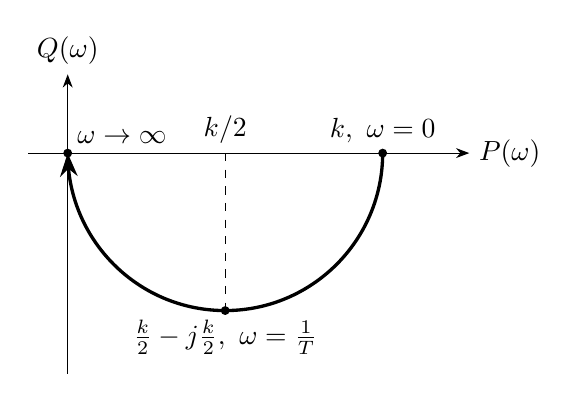
\begin{tikzpicture}[>=Stealth,scale=1.0]
  \draw[->] (-0.5,0) -- (5.1,0) node[right]{$P(\omega)$};
  \draw[->] (0,-2.8) -- (0,1.0) node[above]{$Q(\omega)$};
  \draw[very thick,->] (4,0) arc[start angle=0,end angle=-180,radius=2];
  \fill (4,0) circle (1.6pt) node[above] {$k,\ \omega=0$};
  \fill (2,-2) circle (1.6pt) node[below] {$\frac{k}{2}-j\frac{k}{2},\ \omega=\frac1T$};
  \fill (0,0) circle (1.6pt) node[above right] {$\omega\to\infty$};
  \draw[dashed] (2,0)--(2,-2);
  \node[above] at (2,0) {$k/2$};
\end{tikzpicture}
\end{center}

Biên độ:
\[
\boxed{
A(\omega)=|G(j\omega)|
=\frac{k}{\sqrt{1+T^2\omega^2}}.
}
\]
Pha:
\[
\boxed{
\varphi(\omega)=-\arctan(T\omega).
}
\]
Đặc tính logarithm biên độ:
\[
\boxed{
L(\omega)=20\log_{10}A(\omega)
=
20\log_{10}k
-10\log_{10}\!\left(1+T^2\omega^2\right).
}
\]
Các giá trị đặc trưng:
\[
\omega=0:
\qquad
L(0)=20\log_{10}k,\qquad
\varphi(0)=0,
\]
\[
\omega=\frac1T:
\qquad
L\!\left(\frac1T\right)
=
20\log_{10}\frac{k}{\sqrt2},
\qquad
\varphi\!\left(\frac1T\right)=-\frac{\pi}{4},
\]
\[
\omega\to\infty:
\qquad
L(\omega)\to-\infty,\qquad
\varphi(\omega)\to-\frac{\pi}{2}.
\]

Hình dưới biểu diễn chính xác phần thay đổi do khâu \(1/(Ts+1)\); giá trị \(20\log_{10}k\) chỉ làm tịnh tiến đường biên độ theo phương đứng.

\begin{center}
\begin{tikzpicture}
\begin{axis}[
  width=0.88\linewidth,height=4.6cm,
  xmode=log,xmin=0.01,xmax=100,
  ymin=-42,ymax=3,
  grid=both,
  xlabel={$\omega T$},
  ylabel={$L-20\log_{10}k$ (dB)},
  xtick={0.01,0.1,1,10,100},
  ytick={0,-3.01,-20,-40},
  legend style={font=\small,at={(0.02,0.05)},anchor=south west}
]
\addplot[thick,domain=0.01:100,samples=160]
  {-10*ln(1+x^2)/ln(10)};
\addlegendentry{chính xác}
\addplot[dashed,domain=0.01:1,samples=2] {0};
\addplot[dashed,domain=1:100,samples=80] {-20*ln(x)/ln(10)};
\addlegendentry{tiệm cận}
\addplot[only marks,mark=*] coordinates {(1,-3.0103)};
\end{axis}
\end{tikzpicture}

\begin{tikzpicture}
\begin{axis}[
  width=0.88\linewidth,height=4.2cm,
  xmode=log,xmin=0.01,xmax=100,
  ymin=-95,ymax=5,
  grid=both,
  xlabel={$\omega T$},
  ylabel={$\varphi$ (độ)},
  xtick={0.01,0.1,1,10,100},
  ytick={0,-45,-90}
]
\addplot[thick,domain=0.01:100,samples=160] {-atan(x)};
\addplot[only marks,mark=*] coordinates {(1,-45)};
\end{axis}
\end{tikzpicture}
\end{center}

\baitap{4.4}
\debai
Vẽ đặc tính Nyquist của
\[
G(s)=\frac{4}{1+s}.
\]
Xác định các điểm tại \(\omega=0\), \(\omega=1\), \(\omega\to\infty\).

\loigiai
Thay \(s=j\omega\):
\[
G(j\omega)
=
\frac{4}{1+j\omega}
=
\frac{4}{1+\omega^2}
-j\frac{4\omega}{1+\omega^2}.
\]
Do đó
\[
P(\omega)=\frac{4}{1+\omega^2},
\qquad
Q(\omega)=-\frac{4\omega}{1+\omega^2}.
\]
Các điểm đặc trưng:
\[
G(j0)=4,
\]
\[
G(j1)=2-2j,
\]
\[
G(j\infty)=0.
\]
Quỹ tích thỏa
\[
\boxed{(P-2)^2+Q^2=2^2,\qquad Q\le0.}
\]

\begin{center}
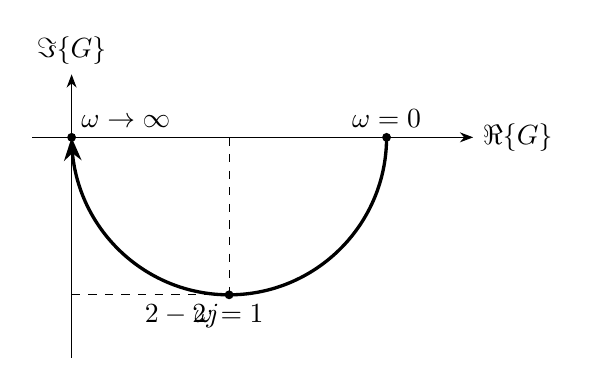
\begin{tikzpicture}[>=Stealth,scale=1.0]
  \draw[->] (-0.5,0)--(5.1,0) node[right]{$\Re\{G\}$};
  \draw[->] (0,-2.8)--(0,0.8) node[above]{$\Im\{G\}$};
  \draw[very thick,->] (4,0) arc[start angle=0,end angle=-180,radius=2];
  \fill (4,0) circle (1.6pt) node[above] {$\omega=0$};
  \fill (2,-2) circle (1.6pt) node[below] {$\omega=1$};
  \fill (0,0) circle (1.6pt) node[above right] {$\omega\to\infty$};
  \draw[dashed] (2,0)--(2,-2);
  \draw[dashed] (0,-2)--(2,-2);
  \node[below left] at (2,-2) {$2-2j$};
\end{tikzpicture}
\end{center}

\baitap{4.5}
\debai
Vẽ đặc tính Nyquist của
\[
G(s)=\frac{3}{s(1+2s)},
\qquad \omega\in(0,\infty).
\]

\loigiai
Thay \(s=j\omega\):
\[
G(j\omega)
=
\frac{3}{j\omega(1+j2\omega)}.
\]
Rút gọn về phần thực và phần ảo:
\[
\boxed{
G(j\omega)
=
-\frac{6}{4\omega^2+1}
-j\frac{3}{\omega(4\omega^2+1)}.
}
\]
Vì vậy
\[
P(\omega)=-\frac{6}{4\omega^2+1},
\qquad
Q(\omega)=-\frac{3}{\omega(4\omega^2+1)}.
\]
Các điểm giới hạn:
\[
\omega\to0^+:
\qquad
P\to-6,\quad Q\to-\infty,
\]
\[
\omega=\frac12:
\qquad
G\!\left(j\frac12\right)=-3-3j,
\]
\[
\omega\to\infty:
\qquad
G(j\omega)\to0.
\]

\begin{center}
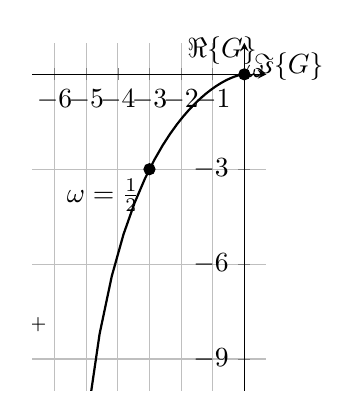
\begin{tikzpicture}
\begin{axis}[
  width=0.72\linewidth,height=6.0cm,
  axis lines=middle,
  xmin=-6.7,xmax=0.7,
  ymin=-10,ymax=1.0,
  xlabel={$\Re\{G\}$},
  ylabel={$\Im\{G\}$},
  grid=both,
  xtick={-6,-5,-4,-3,-2,-1,0},
  ytick={-9,-6,-3,0},
  axis equal image
]
\addplot[thick,domain=0.18:12,samples=240,variable=\w]
  ({-6/(4*\w^2+1)},{-3/(\w*(4*\w^2+1))});
\addplot[only marks,mark=*] coordinates {(-3,-3) (0,0)};
\node[anchor=north east] at (axis cs:-3,-3) {$\omega=\frac12$};
\node[anchor=south east] at (axis cs:-5.9,-8.7) {$\omega\to0^+$};
\node[anchor=south west] at (axis cs:-0.25,-0.4) {$\omega\to\infty$};
\end{axis}
\end{tikzpicture}
\end{center}

\baitap{4.6}
\debai
Vẽ đặc tính logarithm (Bode) của
\[
G(s)=\frac{100}{s+2}.
\]

\loigiai
Đưa về dạng khâu quán tính bậc nhất:
\[
G(s)
=
\frac{100}{2(0.5s+1)}
=
\frac{50}{0.5s+1}.
\]
Suy ra
\[
k=50,\qquad T=0.5,
\qquad
\omega_g=\frac1T=2\ {\rm rad/s}.
\]
Biên độ logarithm và pha:
\[
\boxed{
L(\omega)
=
20\log_{10}
\frac{50}{\sqrt{1+0.25\omega^2}},
}
\]
\[
\boxed{
\varphi(\omega)=-\arctan(0.5\omega).
}
\]
Các điểm đặc trưng:
\[
L(0)=20\log_{10}50\approx33.98\ {\rm dB},
\qquad
\varphi(0)=0,
\]
\[
L(2)
=
20\log_{10}\frac{50}{\sqrt2}
\approx30.97\ {\rm dB},
\qquad
\varphi(2)=-45^\circ,
\]
và khi \(\omega\to\infty\),
\[
L(\omega)\to-\infty,
\qquad
\varphi(\omega)\to-90^\circ.
\]
Đường tiệm cận biên độ nằm ngang ở \(33.98\) dB trước \(\omega_g=2\), sau đó có độ dốc \(-20\) dB/decade.

\begin{center}
\begin{tikzpicture}
\begin{axis}[
  width=0.88\linewidth,height=4.8cm,
  xmode=log,xmin=0.1,xmax=100,
  ymin=-2,ymax=38,
  grid=both,
  xlabel={$\omega$ (rad/s)},
  ylabel={$L(\omega)$ (dB)},
  xtick={0.1,1,2,10,100},
  legend style={font=\small,at={(0.02,0.05)},anchor=south west}
]
\addplot[thick,domain=0.1:100,samples=180]
  {20*ln(50/sqrt(1+0.25*x^2))/ln(10)};
\addlegendentry{chính xác}
\addplot[dashed,domain=0.1:2,samples=2] {20*ln(50)/ln(10)};
\addplot[dashed,domain=2:100,samples=100]
  {20*ln(50)/ln(10)-20*ln(x/2)/ln(10)};
\addlegendentry{tiệm cận}
\addplot[only marks,mark=*] coordinates {(2,30.969)};
\end{axis}
\end{tikzpicture}

\begin{tikzpicture}
\begin{axis}[
  width=0.88\linewidth,height=4.2cm,
  xmode=log,xmin=0.1,xmax=100,
  ymin=-95,ymax=5,
  grid=both,
  xlabel={$\omega$ (rad/s)},
  ylabel={$\varphi(\omega)$ (độ)},
  xtick={0.1,1,2,10,100},
  ytick={0,-45,-90}
]
\addplot[thick,domain=0.1:100,samples=180] {-atan(0.5*x)};
\addplot[only marks,mark=*] coordinates {(2,-45)};
\end{axis}
\end{tikzpicture}
\end{center}

\baitap{4.7}
\debai
Xác định và vẽ đặc tính Bode của
\[
G(s)=\frac{100}{s^2+3s+2}.
\]

\loigiai
Phân tích mẫu:
\[
s^2+3s+2=(s+1)(s+2).
\]
Chuẩn hóa từng khâu:
\[
G(s)
=
\frac{50}{(s+1)(0.5s+1)}.
\]
Có thể xem
\[
G(s)=G_1(s)G_2(s),
\]
với
\[
G_1(s)=\frac{100}{s+1},
\qquad
G_2(s)=\frac{1}{s+2}
=\frac{0.5}{0.5s+1}.
\]
Do các khâu mắc nối tiếp:
\[
\boxed{
L(\omega)=L_1(\omega)+L_2(\omega),
\qquad
\varphi(\omega)=\varphi_1(\omega)+\varphi_2(\omega).
}
\]
Cụ thể:
\[
\boxed{
L(\omega)
=
20\log_{10}50
-10\log_{10}(1+\omega^2)
-10\log_{10}(1+0.25\omega^2),
}
\]
\[
\boxed{
\varphi(\omega)
=
-\arctan(\omega)-\arctan(0.5\omega).
}
\]
Hai tần số gãy:
\[
\omega_{g1}=1\ {\rm rad/s},
\qquad
\omega_{g2}=2\ {\rm rad/s}.
\]
Đường tiệm cận biên độ có:
\begin{itemize}
  \item độ dốc \(0\) dB/decade khi \(\omega<1\);
  \item độ dốc \(-20\) dB/decade khi \(1<\omega<2\);
  \item độ dốc \(-40\) dB/decade khi \(\omega>2\).
\end{itemize}
Pha đi từ \(0^\circ\) về \(-180^\circ\).

\begin{center}
\begin{tikzpicture}
\begin{axis}[
  width=0.88\linewidth,height=4.8cm,
  xmode=log,xmin=0.05,xmax=100,
  ymin=-55,ymax=38,
  grid=both,
  xlabel={$\omega$ (rad/s)},
  ylabel={$L(\omega)$ (dB)},
  xtick={0.1,1,2,10,100},
  legend style={font=\small,at={(0.02,0.05)},anchor=south west}
]
\addplot[thick,domain=0.05:100,samples=200]
  {20*ln(50/sqrt((1+x^2)*(1+0.25*x^2)))/ln(10)};
\addlegendentry{chính xác}
\addplot[dashed,domain=0.05:1,samples=2] {20*ln(50)/ln(10)};
\addplot[dashed,domain=1:2,samples=25]
  {20*ln(50)/ln(10)-20*ln(x)/ln(10)};
\addplot[dashed,domain=2:100,samples=100]
  {(20*ln(50)/ln(10)-20*ln(2)/ln(10))-40*ln(x/2)/ln(10)};
\addlegendentry{tiệm cận}
\end{axis}
\end{tikzpicture}

\begin{tikzpicture}
\begin{axis}[
  width=0.88\linewidth,height=4.2cm,
  xmode=log,xmin=0.05,xmax=100,
  ymin=-185,ymax=5,
  grid=both,
  xlabel={$\omega$ (rad/s)},
  ylabel={$\varphi(\omega)$ (độ)},
  xtick={0.1,1,2,10,100},
  ytick={0,-45,-90,-135,-180}
]
\addplot[thick,domain=0.05:100,samples=200]
  {-atan(x)-atan(0.5*x)};
\end{axis}
\end{tikzpicture}
\end{center}

\end{document}
